\documentclass[
	a4paper,					% paper format
	11pt,							% fontsize
	twoside,					% double-sided
	openright,				% begin new chapter on right side
	notitlepage,			% use no standard title page
	parskip=half,			% set paragraph skip to half of a line
]{scrreprt}					% KOMA-script report

\raggedbottom
\KOMAoptions{cleardoublepage=plain}			% Add header and footer on blank pages
\usepackage[utf8]{inputenc}  							% Unix/Linux - load extended character set (ISO 8859-1)

\usepackage{csquotes}
\usepackage[hidelinks]{hyperref}
\usepackage{color}

% Code Segments
\usepackage{listings}
% Copyright 2017 Sergei Tikhomirov, MIT License
% https://github.com/s-tikhomirov/solidity-latex-highlighting/
\usepackage{listings, xcolor}

\newcommand\YAMLcolonstyle{\color{red}\mdseries}
\newcommand\YAMLkeystyle{\color{black}\bfseries}
\newcommand\YAMLvaluestyle{\color{blue}\mdseries}

\makeatletter

% here is a macro expanding to the name of the language
% (handy if you decide to change it further down the road)
\newcommand\language@yaml{yaml}

\expandafter\expandafter\expandafter\lstdefinelanguage
\expandafter{\language@yaml}
{
  keywords={true,false,null,y,n},
  keywordstyle=\color{darkgray}\bfseries,
  basicstyle=\YAMLkeystyle,                                 % assuming a key comes first
  sensitive=false,
  comment=[l]{\#},
  morecomment=[s]{/*}{*/},
  commentstyle=\color{purple}\ttfamily,
  stringstyle=\YAMLvaluestyle\ttfamily,
  moredelim=[l][\color{orange}]{\&},
  moredelim=[l][\color{magenta}]{*},
  moredelim=**[il][\YAMLcolonstyle{:}\YAMLvaluestyle]{:},   % switch to value style at :
  morestring=[b]',
  morestring=[b]",
  literate =    {---}{{\ProcessThreeDashes}}3
                {>}{{\textcolor{red}\textgreater}}1     
                {|}{{\textcolor{red}\textbar}}1 
                {\ -\ }{{\mdseries\ -\ }}3,
}

% switch to key style at EOL
\lst@AddToHook{EveryLine}{\ifx\lst@language\language@yaml\YAMLkeystyle\fi}
\makeatother

\newcommand\ProcessThreeDashes{\llap{\color{cyan}\mdseries-{-}-}}


\usepackage[standard-baselineskips]{cmbright}

\usepackage[T1]{fontenc}											% hyphenation of words with �,� and �
\usepackage{textcomp}													% additional symbols
\usepackage{ae}																% better resolution of Type1-Fonts 
\usepackage{fancyhdr}													% simple manipulation of header and footer 
\usepackage{etoolbox}													% color manipulation of header and footer

\usepackage[english]{babel}										% english hyphenation
%\usepackage[ansinew]{inputenc}  							% Windows - load extended character set (ISO 8859-1)
\usepackage{graphicx}                      		% integration of images
\usepackage{float}														% floating objects
\usepackage{caption}													% for captions of figures and tables
\usepackage{booktabs}													% package for nicer tables
\usepackage{tocvsec2}													% provides means of controlling the sectional numbering
\usepackage{tabularx}
%---------------------------------------------------------------------------


% Set up page dimension
%---------------------------------------------------------------------------
\usepackage{geometry}
\geometry{
	a4paper,
	left=28mm,
	right=15mm,
	top=30mm,
	headheight=20mm,
	headsep=10mm,
	textheight=242mm,
	footskip=15mm
}


% Compact Itemize:
%---------------------------------------------------------------------------
\newenvironment{compactitemize}
{ \begin{itemize}
    \setlength{\itemsep}{0pt}
    \setlength{\parskip}{0pt}
    \setlength{\parsep}{0pt}     }
{ \end{itemize}                  }
\newenvironment{compactenumerate}
{ \begin{enumerate}
    \setlength{\itemsep}{0pt}
    \setlength{\parskip}{0pt}
    \setlength{\parsep}{0pt}     }
{ \end{enumerate}  				 }

\RequirePackage{color}                          % Color (not xcolor!)
\definecolor{linkblue}{rgb}{0,0,0.8}            % Standard
\definecolor{darkblue}{rgb}{0,0.08,0.45}        % Dark blue
\definecolor{bfhgrey}{rgb}{0.41,0.49,0.57}      % BFH grey
\definecolor{linkcolor}{rgb}{0,0,0.8}  
\definecolor{darkblue}{rgb}{0,.2,.4}
\definecolor{darkgray}{rgb}{.4,.4,.4}
\definecolor{purple}{rgb}{0.65, 0.12, 0.82}
\definecolor{brown}{rgb}{.4,.4,.3}
\definecolor{darkred}{rgb}{.6,0,0}
\definecolor{linenumbergray}{rgb}{.6,.6,.6}   			% Blue for the web- and cd-version!
%\definecolor{linkcolor}{rgb}{0,0,0}        			% Black for the print-version!


\usepackage{colortbl}
\usepackage{longtable}
\usepackage{lscape}


\newcolumntype{L}[1]{>{\raggedright\let\newline\\\arraybackslash\hspace{0pt}}m{#1}}
\newcolumntype{C}[1]{>{\centering\let\newline\\\arraybackslash\hspace{0pt}}m{#1}}
\newcolumntype{R}[1]{>{\raggedleft\let\newline\\\arraybackslash\hspace{0pt}}m{#1}}


% Package to facilitate placement of boxes at absolute positions
%---------------------------------------------------------------------------
\usepackage[absolute]{textpos}
\setlength{\TPHorizModule}{1mm}
\setlength{\TPVertModule}{1mm}

% Sequence Diagram
\usepackage{geometry}
\usepackage{pgf-umlsd}
\usetikzlibrary{calc}

% Glossary
\usepackage[toc,section=section, acronym]{glossaries}
\makeglossaries
\usepackage{glossaries}

\newacronym{cli}{CLI}{comand line interface}
\newacronym{sha256}{SHA-256}{Secure Hashing Algorithm - 256}

\newacronym{ids}{IDS}{intrusion detection system}
\newacronym{apt}{APT}{advanced persistant threat}
\newacronym{fim}{FIM}{file integrity monitoring} 
\newacronym{hids}{HIDS}{host-based intrusion detection system} 
\newacronym{nids}{NIDS}{network-based intrusion detection system} 
\newacronym{nist}{NIST}{National Institute of Standards and Technology}
\newacronym{owasp}{OWASP}{Open Web Application Security Project}
\newacronym{it}{IT}{Information Security}
\newacronym{tb}{TB}{Terrabyte}
\newacronym{mb}{MB}{Megabyte}
\newacronym{kb}{KB}{Kilobyte}
\newacronym{itsec}{ITSec}{\gls{it} Security}
\newglossaryentry{yaml}{name=YAML, description={YAML Ain't Markup Language}}
\newglossaryentry{regex}{name=regex, description={Regular Expressions are a standard way to find certain patterns in a string.}}
\newacronym{tsk}{TSK}{The Sleuth Kit}
\newacronym{tls}{TLS}{Transport Layer Security}
\newacronym{api}{API}{Application Programming Interface}
\newacronym{json}{JSON}{JavaScript Object Notation}
\newacronym{loa}{LoA}{Level of Assurance}
\newacronym{hdd}{HDD}{Hard Disk Drive}
\newacronym{ssd}{SSD}{Solid State Drive}
\newacronym{dbms}{DBMS}{DataBase Management System}
\newacronym{id}{ID}{IDentifier}
\newacronym{uuid}{UUID}{Universaly Unique IDentifier}
\newacronym{cd}{CD}{Compact Disc}
\newacronym{dvd}{DVD}{Digital Versatile Disc}
\newacronym{usb}{USB}{Universal Serial Bus}
\newacronym{ioc}{IoC}{Indicator of Compromise}
\newglossaryentry{sql}{name=SQL, description={A domain specific language used for querying a relational database.}}
\newglossaryentry{unixts}{name=UNIX timestamp, description={The number of seconds since 00:00:00 on the 1st of January 1970}}
\newglossaryentry{hex}{name=hexadecimal, description={A number system with 16 digits. It uses the numbers 0-9 and the Letters A-F.}}


\newglossaryentry{pgp}{type=\acronymtype, name={PGP}, description={Pretty Good Privacy}, first={Pretty Good Privacy (PGP)\glsadd{pgpg}}, see=[Glossary:]{pgpg}}
\newglossaryentry{}{name=, description={}}
\newglossaryentry{pgpg}{name=PGP, description={Standard for encryption and signatures defined in RFC4880}}
\newglossaryentry{postgres}{name=postgres, description={An opensource database server. It is rather lightweight and heavily used.}}
\newglossaryentry{sqlite}{name=sqlite, description={A very lightweight relational database implemnentation. It does not have a dedicated server but instead writes the database to a file which is written to the local host.}}
\newglossaryentry{opensource}{name=opensource, description={Software where both the source and the software is freely accessible and changable.}}
\newglossaryentry{github}{name=github, description={A platform for \gls{opensource} projects. It is free to use and hosts the source code for many projects.}}
\newglossaryentry{storagemedia}{name=storage media, description={media that is used to store data in a computer system.}}
\newglossaryentry{malware}{name=malware, description={Malware is any program that is designed to harm a computer system. The term includes well known terms like Virus, Worm, Adware, Keylogger, Trojan, etc. Malware usually tries to hide it's traces to achieve longer infection periods of time. }}
\newglossaryentry{collision}{name=collision, plural=collisions, description={Multiple different inputs with the same hash value.}}

\newglossaryentry{anomaly}{
name=anomaly, 
plural=anomalies,
description={An unexpected change in the file system. For a change to be unexpected it needs to be covered by the configuration changes are unexpected only if the configuration says so. Some examples that might cause anomalies, changed rights, new files, deleted files. }}
\newglossaryentry{intrusion}{
name=intrusion, 
plural=intrusions,
description={An unauthorized access to a system or to data. }}
\newglossaryentry{investigation}{
name=investigation, 
plural=investigations,
description={The process of finding out what exactly happened after an incident.}}
\newglossaryentry{hash}{
name=cryptographic hash function, 
plural=cryptographic hash functions,
description={A deterministic one way function that fullfills collision resistance and other cryptographic properties. Implementations are the SHA-2 and SHA-3 families.}}
\newglossaryentry{nonhash}{
name=non-cryptographic hash function, 
plural=non-cryptographic hash functions,
description={A deterministic one way function that does not the hard to achieve properties that make a \gls{hash}. Often used when speed is more important than collision resistance.}}
\newglossaryentry{fs}{
name=file system, 
description={A file system is used to create a layer of abstraction between the hardware of the storage medium and the operating system. There are multiple file system types which are in use with different capabilities. Additionally to the files the file systems keep track of meta data to each file. This meta data includes some timestamps (created, last accessed, etc) and more.}}
\newglossaryentry{pytsk}{name=pytsk3, description={Python bindings for \gls{tsk}}}
\newglossaryentry{metadata}{name=metadata, description={Data that gives information on other data. In this thesis it is mostly used to describe attributes of the \gls{fs} that describes files. Exmaples are creation date and permissions.}}
\newglossaryentry{git}{name=git, description={A distributed version-control system used for source code tracking in software engineering. Nicknamed \'the stupid content tracker\', stands for either \'global information tracker\' or \'goddamn idiotic truckload of s...\'}}








\usepackage{polyglossia}
\setdefaultlanguage{english}
\usepackage[backend=biber]{biblatex}
\addbibresource{database/thesis.bib}
\usepackage{pgfgantt}


\definecolor{ganttplanned}{RGB}{0,80,200}
\definecolor{ganttplannedopt}{RGB}{50,50,50}
\definecolor{ganttactual}{RGB}{234,187,0}
\definecolor{ganttunplanned}{RGB}{153,0,0}

\newganttchartelement*{plannedmilestone}{%
  plannedmilestone/.style={
	shape=ganttmilestone,
	inner sep=0pt,
	draw=ganttplanned!50!black,
	top color=white,	
	bottom color=ganttplanned!50% 
  },
  plannedmilestone label text=\strut#1,
  plannedmilestone label font=\footnotesize,
  plannedmilestone label node/.style={%
	anchor=east, font=\ganttvalueof{plannedmilestone label font}%
  },%
  plannedmilestone inline label anchor=center,%
  plannedmilestone inline label node/.style={%
	anchor=south, font=\ganttvalueof{plannedmilestone label font}%
  },%
  plannedmilestone left shift = .6,
  plannedmilestone right shift = .4,
  plannedmilestone top shift = .05,
  plannedmilestone height = .6
}
\newganttchartelement*{actualmilestone}{%
  actualmilestone/.style={
	shape=ganttmilestone,
	inner sep=0pt,
	draw=ganttactual!50!black,
	top color=white,	
	bottom color=ganttactual!50% 
  },
  actualmilestone label text=\strut#1,
  actualmilestone label font=\footnotesize,
  actualmilestone label node/.style={%
	anchor=east, font=\ganttvalueof{actualmilestone label font}%
  },%
  actualmilestone inline label anchor=center,%
  actualmilestone inline label node/.style={%
	anchor=south, font=\ganttvalueof{actualmilestone label font}%
  },%
  actualmilestone left shift = .6,
  actualmilestone right shift = .4,
  actualmilestone top shift = .35,
  actualmilestone height = .6
}





\begin{document}


\settocdepth{section}														% Set depth of toc
\pagenumbering{roman}														
%---------------------------------------------------------------------------

\providecommand{\heading}{Alternative scalable HIDS with investigation capability}		%  Insert Title of Thesis here					% Titel der Arbeit aus Datei titel.tex lesen
\providecommand{\versionnumber}{1.0.1}			%  Hier die aktuelle Versionsnummer eingeben
\providecommand{\versiondate}{\today}		%  Hier das Datum der aktuellen Version eingeben				% Versionsnummer und -datum aus Datei version.tex lesen

% Set up header and footer
%---------------------------------------------------------------------------
\makeatletter
\patchcmd{\@fancyhead}{\rlap}{\color{bfhgrey}\rlap}{}{}		% new color of header
\patchcmd{\@fancyfoot}{\rlap}{\color{bfhgrey}\rlap}{}{}		% new color of footer
\makeatother

\fancyhf{}																		% clean all fields
\fancypagestyle{plain}{												% new definition of plain style	
	\fancyfoot[OR,EL]{\footnotesize \thepage} 	% footer right part --> page number
	\fancyfoot[OL,ER]{\footnotesize \heading, Version \versionnumber, \versiondate}	% footer even page left part 
}

\renewcommand{\chaptermark}[1]{\markboth{\thechapter.  #1}{}}
\renewcommand{\headrulewidth}{0pt}				% no header stripline
\renewcommand{\footrulewidth}{0pt} 				% no bottom stripline

\pagestyle{plain}
%---------------------------------------------------------------------------


% Title Page and Abstract
%---------------------------------------------------------------------------
%
% Project documentation template
% ===========================================================================
% This is part of the document "Project documentation template".
% Authors: brd3, kaa1
%

\begin{titlepage}


% BFH-Logo absolute placed at (28,12) on A4 and picture (16:9 or 15cm x 8.5cm)
% Actually not a realy satisfactory solution but working.
%---------------------------------------------------------------------------
\setlength{\unitlength}{1mm}
\begin{textblock}{20}[0,0](28,12)
	
\includegraphics[scale=1.0]{../img/BFH_Logo_B.png}
\end{textblock}

% Institution / titel / subtitel / authors / experts:
%---------------------------------------------------------------------------
\begin{flushleft}

\vspace*{21mm}

\fontsize{26pt}{40pt}\selectfont 
\heading				\\							% Read heading from file leader/title.tex
\vspace{2mm}

\fontsize{16pt}{24pt}\selectfont\vspace{0.3em}
Forensic-based intrusion detection system	(FIDS)		\\				% Insert subheading
\vspace{5mm}

\fontsize{10pt}{12pt}\selectfont
\textbf{Bachelor thesis} \\		% Insert text
\vspace{7mm}

% Abstract (eingeben):
%---------------------------------------------------------------------------
\begin{textblock}{150}(28,100)
\fontsize{10pt}{12pt}\selectfont
In this thesis, I show how a host-based intrusion detection system can be built for scalability. More specifically, I show how the sleuth kit can be used to create an intrusion detection system that does not rely on hashing, but on filesystem attributes. This way, it gains speed, which enables us to take the risk not to calculate hashes.
\end{textblock}

\begin{textblock}{150}(28,225)
\fontsize{10pt}{17pt}\selectfont
\begin{tabbing}
xxxxxxxxxxxxxxxxxxxxx\=xxxxxxxxxxxxxxxxxxxxxxxxxxxxxxxxxxxxxxxxxxxxxxx \kill
Degree programme:	\> BSc in Computer Science	\\		% insert name of degree course
Specialisation:	\> IT Security	\\		% insert name of degree course
Author:		\> 		Julian Stampfli\\					% insert names
Tutor:	\> Dr.~Bruce Nikkel		\\							% insert names
Expert:		\> Armin Blum				\\							% insert names
Date:			\> \versiondate					\\							% read from file leader/version.tex
\end{tabbing}

\end{textblock}
\end{flushleft}

\begin{textblock}{150}(28,280)
\noindent 
\color{bfhgrey}\fontsize{9pt}{10pt}\selectfont
Berner Fachhochschule | Haute \'ecole sp\'ecialis\'ee bernoise | Bern University of Applied Sciences
\color{black}\selectfont
\end{textblock}


\end{titlepage}

%
% ===========================================================================
% EOF
%
		% activate for frontpage without picture
%\include{leader/frontpage_with_picture}		% activate for frontpage with picture
\cleardoubleemptypage
\setcounter{page}{1}
\cleardoublepage
\phantomsection 
\addcontentsline{toc}{chapter}{Abstract}
\chapter*{Abstract}
\label{chap:abstract}

Lorem ipsum dolor sit amet, consectetur adipiscing elit. Phasellus scelerisque, leo sed iaculis ornare, mi leo semper urna, ac elementum libero est at risus. Donec eget aliquam urna. Lorem ipsum dolor sit amet, consectetur adipiscing elit. Nunc fermentum nunc sollicitudin leo porttitor volutpat. Duis ac enim lectus, quis malesuada lectus. Aenean vestibulum suscipit justo, in suscipit augue venenatis a. Donec interdum nibh ligula. Aliquam vitae dui a odio cursus interdum quis vitae mi. Phasellus ornare tortor fringilla velit accumsan quis tincidunt magna eleifend. Praesent nisl nibh, cursus in mattis ac, ultrices ac nulla. Nulla ante urna, aliquet eu tempus ut, feugiat id nisl. Nunc sit amet mauris vitae turpis scelerisque mattis et sed metus. Aliquam interdum congue odio, sed semper elit ullamcorper vitae. Morbi orci elit, feugiat vel hendrerit nec, sollicitudin non massa. Quisque lacus metus, vulputate id ullamcorper id, consequat eget orci \nocite{kopka:band1} \nocite{Marti06}. 

\cleardoubleemptypage
\phantomsection 
\addcontentsline{toc}{chapter}{Acknowledgements}
\chapter*{Acknowledgements}
\label{chap:acknowledgements}

Firstly, I want to tank my tutor Bruce Nikkel and for his outstanding guidance and ongoing support during this project.

Next, I want to thank Amir Blum for supervising this work as my expert and for giving valuable feedback at the start of the project.

Further, I want to thank the \gls{opensource} community behind \gls{tsk} and \gls{pytsk} without whom this project would not have been possible. Especially Joachim Metz who is very active in the \gls{pytsk} community and helped me find the solution to one of my issues.

\cleardoubleemptypage
%---------------------------------------------------------------------------

% Table of contents
%---------------------------------------------------------------------------
\tableofcontents
\cleardoublepage
%---------------------------------------------------------------------------

% Main part:
%---------------------------------------------------------------------------
\pagenumbering{arabic}

\chapter{Introduction}

Attacks on computer systems have become highly prevalent. This situation resulted in the creation of many tools that support the securing of said computer systems. Those tools have different purposes and are grouped into different families. Some of those families are responsible for keeping any malicious activity outside of the network while others try to find out whenever something manages to come through. Those types of system are named \gls{ids}. An \gls{ids} generally works by tracking and evaluating some form of activity from hosts and networks and then tries to find \glspl{anomaly}. They operate by comparing the current activity to some configuration which usually contains a form of a whitelist and blacklist. Found \glspl{anomaly} are then alerted or logged such that investigators and system administrators can evaluate the \gls{anomaly} and depending on the result of the evaluation, take action. \cite{hidsnids}

There are two flavors of \gls{ids}, one, which deals with data from the network, named \gls{nids}, and another which evaluates data from the host system, named \gls{hids}. \gls{nids} are used to detect unusual behavior of the network like communication from hosts which usually don't communicate or suspiciously large amounts of data that is transferred. \gls{hids}, on the other hand, are used to detect \glspl{anomaly} on a host. This process works by detecting changes like which processes are started or when the \gls{fs} is changed. Both types of \gls{ids} have various advantages, and they should be used in conjunction for best results. \cite{hidsnids}

This thesis is about the writing of a \gls{hids} by analyzing changes on the \gls{fs} through \gls{fim}. As already mentioned, a \gls{hids} operates on the host machine and detects \glspl{anomaly} by comparing resources available on the host. For \gls{fim} a \gls{hids} usually calculates a \gls{hash} for each file and compares them to previous executions. If the output of the \gls{hash} changes, then the file has been altered. If this alteration is unexpected and detected as an \gls{anomaly} by comparing it to a configuration, it is alerted. This approach has one weakness. The calculation of a \glspl{hash} takes time.

Additionally, to calculate the hash function, the \gls{hids} needs to read the whole content of the relevant files. Because those files are stored on some \gls{storagemedia}, it takes even more time for the whole process of reading the file from the \gls{fs} and calculating the hash \cite{hash:slow, hash:speed}. This issue is, from a historical perspective, not relevant, as it was efficient enough that the entire \gls{fs} could be hashed in a small amount of time. However, \glspl{storagemedia} grew, and with it, the amount of data on a host \cite{bruce:imaging}. With that, the calculation of \glspl{hash} needs more time. So much indeed, that traditional \gls{hids} can't scan big systems within a valuable amount of time anymore.

There is another way. Instead of reading the entire file and calculating the hashes for each, the \gls{fs} already contains some information that can be valuable for \gls{fim}. The \gls{fs} contains much \gls{metadata}. Things like modification date, permissions, and file size. Accessing this type of information is cheap, and it can be achieved without touching any contents within the file. This data can be used for \gls{fim} and finally, to find \glspl{anomaly} \cite{inode}. While not as reliable as hashing, the speed gain can justify sacrificing a small fraction of reliability. This risk has to be considered because finding an \gls{intrusion} fast can be the difference between an attempted \gls{intrusion} and a successful attack with possible exfiltration of data. 

Another advantage that this \gls{hids} has is the built-in support for forensic investigations. Sometimes it is not sufficient to find \glspl{intrusion}, because every \gls{ids} can miss some \glspl{intrusion} which then need manual investigation. For those investigations to be successful, more data is better because it makes it easier to reconstruct the attack. This way, they can evaluate what has happened and assess the risk. Most \gls{hids} solutions don't offer much help in this regard. The solution developed within this thesis, however, has this idea of a forensic investigation built-in.


\chapter{Technical Background}

In this chapter, I provide some technical introduction to relevant topics. Further information is available in the linked resources.

\section{Definitions}

\subsection{Filesystem}
\label{sec:fs}

\gls{storagemedia} takes many forms. There are the traditional \gls{hdd} and newer \gls{ssd}. Both are built based on different assumptions and using different technologies. There exist more \gls{storagemedia} like \gls{cd}, \gls{dvd}, \gls{usb} flash drives and more. \gls{storagemedia} operates on blocks of data. One such block is typicaly 512 bytes or 4 \gls{kb}. \cite{bruce:imaging}

An operating system typically needs to store files of data. This is where \glspl{fs} come in. They create a layer of abstraction for the \gls{storagemedia}. A \gls{fs} uses the blocks of the \gls{storagemedia} and stores the files in a data structure called inode \cite{inode}. The \gls{fs} also keeps track of \gls{metadata} like creation time, accessed time, permissions, etc. Which \gls{metadata} is stored depends on the \gls{fs}. \cite{bruce:imaging}

\subsection{Cryptographic Hashing Function}
\label{sec:hashing}

A hash function is, in general, a function which takes an input of unspecified size and generates an output of a fixed size. Hash functions are used widely in programming and databases to access certain data within a data structure easily. By design, hash functions have \glspl{collision}, meaning that multiple inputs generate the same output. This statement must be true if you consider the unlimited input size and limited output size. If there are more inputs than outputs, there must be at least one value that is assigned to multiple inputs. For data storage and other use cases this is not a huge problem because collisions can be handled, and if the hash function has good distribution, collisions are unlikely. Additionally, in many systems, a hashing function with weak collision resistance is deliberately chosen because it is faster to execute. \cite{hash:noncrypto, hash:slow}

In a cryptographic context, this tradeoff cannot be taken. Two big factors play into why not. Firstly in cryptography hashes are often used as an assurance that the content of some data has not changed. If collisions are easy to find, the data can be altered in ways that result in the same hash, meaning that the hash no longer fulfills the use case. Additionally, potential gain can be big. If a collision can be provoked, even if challenging, data can be changed. This data could be a legal document or a bank transaction, neither of which we want to change. For those reasons, a cryptographic hash function needs to be highly collision resistant. The drawback of collision resistant algorithms over easier hashing functions are operations needed for the calculation, while current hashing functions are performant and secure, they still take some time for much data. \cite{crypto}

One \gls{hash} is called \gls{sha256}. \gls{sha256} is a standard published by the \gls{nist}. It creates a 256-bit output and has not yet been successfully attacked. \cite{sha} This hashing algorithm is used to make sure that the configuration of this implementation has not changed between multiple runs.


\subsection{HIDS}
\label{sec:def:hids}

A \gls{hids} works by detecting changes on the local host. It does that by looking at files, processes, configuration, logs, or other indicators. In this thesis, I focus on files. It is important to note that the other sources are a valuable source of information. Any of those sources might have signs of intrusions. Especially running processes and the configuration can hold relevant data. However, this implementation only covers file-based information due to the lack of resources.

In a \gls{hids} that operates on the \gls{fs}, all the valuable information comes from unexpected changes to the \gls{fs}. Most hosts do not have any changes on the \gls{fs} except for software updates. Additionally, the \gls{fs} usually contains too much information to cover in a handwritten configuration. Thus, the easiest approach is to compare the current state of the \gls{fs} to previous ones. If it has changed significantly or in an unexpected way, something foul might be happening. The negative side effect of this approach is the false positives that come from legitimately changing the host. Those legitimate changes could be new versions of the webpage that is running, newly updated configuration or updated ssh keypairs. However, those changes come scheduled, and the alerts can then be quickly checked and acknowledged.

A good \gls{hids} should be able to handle such valid changes without much change. Additionally, it should be able to find intrusions reliably and in a timely fashion. Maybe it is too late if the \gls{hids} finds an intrusion a week after it infected the system. To detect changes on the files reliably popular \gls{hids} calculate a hash of the files and compares that hash to previous runs. If a \gls{hash} is used, each file always generates a unique hash which can not be forged. The main drawback of using good \glspl{hash} is that they take a longer time. Some implementations thus use weaker implementations of \gls{hash} or even \gls{nonhash}. The obvious drawback of this approach is that a collision can be generated and such a file can be altered or replaced without the \gls{hids} noticing.

In the following sections, I present two of the most used \gls{hids}, Tripwire, and Aide. They built the main competition of the integration developed in this thesis.

\subsubsection{Tripwire}
\label{sec:tripwire}

In 1992 the first \gls{hids} named tripwire was created and publicly released as a free tool. In 1997 the creator of tripwire then created the company Tripwire Inc. and bought the naming rights for tripwire. The free version was monetized, and they released new versions of tripwire. \cite{Tripwire:Impl, Tripwire:company} Now they mostly market to enterprise and industrial customer and have more products than only one for file integrity. \cite{tripwire}

As it is a commercial product, it is hard to see how they work in detail since most of the information is only available to paying customer. 

\subsubsection{AIDE}
\label{sec:aide}

Aide is an \gls{opensource} alternative to tripwire. It was created after tripwire went commercial. \cite{aide:totherescue, aide:github}

When aide is first executed, it generates a reference database. This database contains all the information for each file that is within a path of interest. Depending on the config it contains more or less information, including \glspl{hash}. Each subsequent execution then compares the files found to this initially created database. The database needs to be updated manually if the system has a scheduled change. It generates a log of all the changes and distributes that per email or similar depending on the configuration. Both the configuration and the database are usually stored on the file system that is scanned. \cite{aide, aide:doc}

Aide can compare multiple \glspl{hash} and \glspl{nonhash} and some \gls{metadata}. It runs on many modern Unix system \cite{aide} and uses GPG keys to sign their releases. It has a strong community behind it, but only offers a \gls{cli} and has no fancy user interface and is written in C. \cite{aide:github} 


\subsection{NIDS}
\label{sec:def:nids}

Compared to a \gls{hids}, a \gls{nids} can be used to detect intrusions over multiple hosts. \gls{nids} are used to analyze anomalies on the network. An \gls{anomaly} might be an unexpected session from a server which usually doesn't communicate with the internet or unusually large or frequent traffic. Certain intrusions can be tracked by analyzing the content of the packages. Some intrusions are easier to detect on the network. Especially such ones that extract much data or are very aggressive at spreading within a network. The main advantage here is that multiple sources can be combined on the network level. Another advantage this approach has is that current \gls{malware} almost always contains some network communication \cite{Malware:Behaviour,nids}.

However, a \gls{nids} doesn't only have advantages. Certain kinds of attacks can only be detected on the network with much difficulty. For a corrupted file upload cannot be detected by only checking the network. For best results, both types of \gls{ids} can be used in conjunction to detect attacks. 

In this thesis \gls{nids} are not in the center. The implementation doesn't look at network traffic or mimic other \gls{nids} functionality. However, as mentioned above, I highly encourage everyone to use an appropriate \gls{nids} to improve the chance to find an intrusion. 

\subsection{The Sleuth Kit}
\label{sec:tsk}

\gls{tsk} is an \gls{opensource} toolkit used to investigate disk images. It is based on the coroner's toolkit \cite{tct} and contains multiple command line interfaces and an \gls{api} for various purposes. \cite{tsk, tsk:about} It is mainly written in C, runs on Linux, OsX, Windows and more and can be used to analyze many different \glspl{fs}. It is heavily used in forensic investigations to find deleted or corrupted files and for other information gatherings on a disk image.

\subsubsection{fls}
\label{sec:fls}

One of those command line tools is fls. It can be used to access directories, files, and the attributes of each. With it, the directories can be displayed recursively, and for each file, the attributes can be printed to the console. \cite{tsk:fls} This tool plays a central part in this thesis as it is used to recover all the files and attributes to detect intrusions. On how exactly it is used, please refer to section. \ref{sec:Scanner}

\subsection{Python}
\label{sec:python}

Python was the programming language of choice for this product. Python offers many advantages over other languages. Some of those are:

\begin{itemize}
    \item Platform independent
    \item Good community support in the forensic community
    \item Active library for \gls{tsk}
    \item Small overhead
    \item Easy for prototyping
    \item Easy to read
\end{itemize}

This decision was not made very lightly. Other programming languages were considered. For more information on those refer to section \ref{sec:decisions:language}.

\subsubsection{pytsk3}
\label{sec:pytsk3}

Pytsk3 is the library mentioned above that creates bindings for python to the \gls{api} of \gls{tsk}. As \gls{tsk} this library is \gls{opensource} and is still active. It is hosted on \gls{github} and offers most of the functionality of the \gls{tsk} \gls{api}. Pytsk3 is used extensively in the scanner part of the implementation. For further information refer to section \ref{sec:Scanner}.

\section{Proposed solution}
\label{sec:hids}

The main principle behind a \gls{hids} is the detection of changed files. As already discussed in section \ref{sec:def:hids}, most tools rely on the calculation of hashes. This is generally a good approach since changes can be found very reliably; however, as already mentioned, it can drastically hinder the performance of the \gls{hids}. Sadly the actual performance lost cannot be clearly stated, as it heavily depends on what hardware is in use. However, considering the computational overhead of calculating a \gls{hash} it is clear that the time it takes grows with bigger \glspl{fs}. As \gls{storagemedia} has grown from a \gls{mb} to \gls{tb} so has the requirement to store more data. Creating hashes over such big systems is not viable as it can take a long time to create a hash of big amounts of data. \cite{hash:slow, hash:veryslow, hash:speed}

\subsection{Time issues}

In this thesis, I propose a different approach. Ignore the hashing and the file content and focus on the \gls{fs} \gls{metadata} instead. This approach should be sufficient to find intrusions and thanks to not creating hashes, the \gls{hids} can execute more often. If a conventional \gls{hids} might take several days to complete a run on a \gls{fs} with multiple \gls{tb} of data, the proposed approach would take some minutes to hours. It could then be run multiple times a day and find new and changed files within a short amount of time. It is possible that the \gls{hids} misses some changes if the attacker can change all the relevant \gls{metadata} before the system rechecks the same file, but this is a risk that has to be taken to gain the opportunity to scan large \gls{fs}. It is also possible to scan highly critical sections of a system with a traditional \gls{hids} and the rest with the proposed solution. This way, one has both advantages. The whole system can be checked in a timely fashion with the proposed solution, and for certain smaller parts of the system, a general \gls{hids} can detect changes by using strong \glspl{hash}.

This solution uses \gls{tsk} via \gls{pytsk} to extract the \gls{fs} \gls{metadata}. The main advantage that this gives is the interoperability with different \glspl{fs}. Additionally, by directly accessing the attributes from the \gls{fs}, no \gls{metadata} is changed. The files themselves are never touched. Furthermore, it can also be used to get the files and attributes of an image that has been extracted or of a virtual machine. 

\subsection{Investigation capabilities}
\label{sec:investigation:capabilities}
Another improvement upon existing \gls{hids} proposed is that investigation capabilities need to be built in from the start. Traditional \gls{hids} are good at finding intrusions and alerting them. However, they don't offer support for the investigation of the incident. They don't have information beyond what was configured. This lack of information makes sense is dangerous \gls{hash}. If something was missed in the configuration, an investigator can't use the output of those systems to gain further knowledge. They only have the alerts and nothing further.

This solution stores all the available \gls{metadata} for each scanned file for each run. This way, an investigator can use this output to gain more information about how the attacker proceeded. He can look at the changes of permissions, modification of files, even if the alerts might have been ignored. It is also possible to generate a timeline out of this data to form an extended view on what happened when on the \gls{fs}. 

\subsection{Flexibility}

Aide works by comparing runs to one first execution. This is practical as it detects one intrusion multiple times. However, it generates many messages, and users are then less likely to take them seriously. Additionally to that, after a legitimate change to the system, aide always generates alerts until the initial run is reset. This can lead to undetected intrusions a short time after an upgrade, which might also be the most critical window for an intrusion because the update might have created a security risk. Thus, it is possible that an intruder can gain access shortly after an update which is alerted by aide, but ignored because of the false positives.

The proposed system does not have this issue, at least not as strongly. As all the data gets collected for each run, it makes sense to compare each run to the previous. This has the benefit of legitimate changes being adopted into the accepted one run after it has been finished. This results in overall fewer messages, which increases the importance of each. If it is required that the system should always compare against one specific run, this could also clearly be done. The system would need to be configured to not check against the latest, but a specific, predefined run. Only the configuration would then need to be changed to update this predefined run. 

\section{Scope}

In this project I create a \gls{hids} which uses \gls{tsk} to detect changes. It covers the three main changes discussed in section \ref{sec:hids}. This service uses a \gls{sql} database to store the executed runs. It includes user documentation and this thesis documentation. 

Out of scope is the creation of the timeline mentioned in section \ref{sec:investigation:capabilities}. Also, out of scope are extensive alerting functionality and extensive example configurations for commonly used operating systems and tools. Furthermore, any big data analysis of the runs, while very interesting, are also out of scope.


\include{chapter/30results}

\chapter{Results}

In this chapter, I will talk more about the implementation details of the \gls{fids}. I will also look into the security of this implementation and what measures can be implemented to improve it. 

\section{System Architecture}
\label{sec:Architecture}

\begin{figure}[ht]
	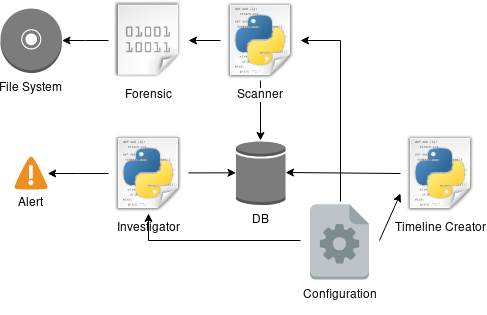
\includegraphics[width=8cm]{../img/Overview_FIDS.png}
	\centering
	\caption{System Architecture}
	\label{fig:systemArchitecture}
\end{figure}

As seen in figure \ref{fig:systemArchitecture}, the \gls{fids} contains two main components, the scanner and the investigator, a database and has connections to some libraries. It is split into scanner and investigator way to gain flexibility, mainly so that both components can be executed independently. This independence has the advantage that the scanner and the investigator don't need to be run on the same system. Also, it means that previous results of the investigator can be recreated by running the investigator on previously captured data. Additionally, if someone is only interested in the results of the scanner, the investigator doesn't need to be run. The scanner is explained in detail in section \ref{sec:Scanner} and the investigator in section \ref{sec:Investigator}.

Additionally, there is the timeline creator. This is another small component which takes the database and creates an output for timelining tools. As such it is not part of the automated \gls{hids} process but offers a human interface for investigation. This is explained in section \ref{sec:Timeliner}. 

Besides the scanner, the investigator and the timeline creator, which were produced in this thesis, there are five other components which build the environment of the \gls{fids}. There is the \gls{fs} which contains the data in which we are interested. As already mentioned, this could be a mounted device that is directly accessible through the operating system. It could also be run on the disk images of virtual machines or previously created disk images. To run it on a previously created disk image might be interesting if used on backup images if backups are made by creating disk images. 

Then there is the forensic component. This component is the combination of \gls{tsk} and \gls{pytsk}. The main purpose of this component is the abstraction of the \gls{fs} into python classes, which can then be used within the scanner. This abstraction is important to be compatible with multiple different \glspl{fs}. \gls{tsk} offers much different functionality; the \gls{fids} is only using the utility that is used for the fls command described in section \ref{sec:fls}. 

This leaves the configuration and the database. Both of which are also part of this thesis. The database is used to store the data of each run, and the configuration is used to change the behavior of the \gls{fids}. The configuration is explained in depth in section \ref{sec:Configuration} and the database in section \ref{sec:Database}.

\subsection{Configuration}
\label{sec:Configuration}

The configuration file is provided in \gls{yaml}. \gls{yaml} is a human-friendly data serialization language with support for many programming languages. Its main advantage over other languages for configuration files is the readability and the ease to extend already existing configuration files. There were more reasons why \gls{yaml} is used documented in appendix section \ref{sec:decisions:config:language}.

\subsubsection{Database Configuration}

The configuration consists of three parts. The first part is the database configuration. The current implementation supports only \gls{sqlite}, as this is the most basic and easy to use format. Additionally, it doesn't require any connection to an external entity. For more information on why \gls{sqlite} was chosen see appendix section \ref{sec:decisions:dbms}. For the configuration, only the filename is required as seen in listing \ref{lst:cfg:sqlite}. This configuration defines where the data will be sent to and read from in the scanner and investigator parts, respectively. As both parts need access to the database, this part of the configuration is in a separate part. It is possible and already prepared to extend the system to use more \gls{dbms}. However, this is not part of the scope of this thesis.

\begin{lstlisting}[language=yaml, numbers=left, caption=SQLite Configuration, label=lst:cfg:sqlite]
sqlite:
	filename: fids_db3.db
\end{lstlisting}

\subsubsection{Scanner Configuration}

The second part of the configuration is the part that defines the scanner. An example config can be seen in listing \ref{lst:cfg:scanner}. It consists of one main key, which is named scan. If this config entry is missing, the scanner part of the \gls{hids} is not executed by default. Beneath this top key it contains the following subkeys:

\begin{description}
	\item [image\_path] Path to the \gls{fs} that is used for the scan.
	\item [scan\_paths] List of paths to scan. Paths are scanned recursively. "/" thus scans all available paths.
	\item [ignore\_paths] Paths that should not be scanned. Can be any directory. The recursion stops once this path is reached and does not continue downwards. Practical if certain directories are not interesting for \gls{intrusion} detection.
\end{description}

\begin{lstlisting}[language=yaml, numbers=left, caption=Scanner Configuration, label=lst:cfg:scanner]
scan:
	image_path: /dev/nvme0n1p1
	scan_paths: 
		[
			"/",
			"/nonExisting",
		]
	ignore_paths: 
		[
			"/temp/"
		]
\end{lstlisting}

\subsubsection{Investigator Configuration}
\label{sec:conf:investigator}

The investigator configuration is similar to the scanner configuration in the way that it contains a top-level node called investigator. If this is missing the investigator part does not start. As can be seen in listing \ref{lst:cfg:investigator} it is a lot more complicated than the scanner configuration. 

\begin{description}
    \item [same\_config] This configuration specifies whether a changed config should result in an alert. Defaults to True.
    \item [validation\_run] This can define a run that is used for validation. If empty the second last one will automatically be used.
    \item [\nameref{sec:config:rules}] Rules are ways to create templates on how changed files should be found. \nameref{sec:config:rules} are explained more through below.
    \item [\nameref{sec:config:investigations}] Investigations define which paths and which files should be checked for \glspl{intrusion}. \nameref{sec:config:investigations} are explained more through below.
\end{description}

\begin{lstlisting}[language=yaml, numbers=left, caption=Investigator Configuration, label=lst:cfg:investigator]
investigator:
	same_config: True
	validation_run: 
	rules: 
		- name: php
		  rules: 
			- m
			- i
			- l
			- n
			- a
		  equal:
			- meta_creation_time
			- meta_size
		- name: logs
		  greater:
			- meta_size
		  equal:
			- meta_creation_time
	investigations:
		- paths:
			- '/etc'
		  whitelist_inverted: false
		  fileregexwhitelist:
			- '*.php'
		  rules:
			- php
		- fileregexwhitelist: '/*'
		  fileregexblacklist: '*evilfile*'
		  blacklist_inverted: false
		  rules:
			- logs
\end{lstlisting}

\subsubsection{Rules}
\label{sec:config:rules}

Rules represent templates that are later used in the investigations to find anomalies. Rules can be based upon other rules to extend them. Recursive rules are allowed, they simply extend each other. An example of the rule configuration can be seen in listing \ref{lst:cfg:investigator}, the fields are explained below.

\begin{description}
	\item [name] Each rule has a name. If two rules with the same name are defined, the behavior might be inconsistent. The name is used to extend rules.
	\item [rules] The rules which are used as a basis for this rule. They are referenced by name.
	\item [greater] The properties which are allowed to grow between the runs. Greater also includes equal.
	\item [equal] The properties that are supposed to stay equal during all runs.
\end{description}

Additionally, there are some predefined rules. The aide configuration heavily influenced which rules got predefined. The preconfigured rules are listed in listing \ref{lst:cfg:precon}.
\begin{lstlisting}[language=yaml, numbers=left, caption=Preconfigured Rules, label=lst:cfg:precon]
rules: 
	- name: p
	  equal:
		- meta_mode
	- name: ftype
	  equal:
		- meta_conten
	- name: i
	  equal:
		- meta_addr
	- name: l
	  equal:
		- meta_link
	- name: n
	  equal:
		- meta_nlink 
	- name: g
	  equal:
		- meta_gid
	- name: s
	  equal:
		- meta_size
	- name: m
	  equal:
		- meta_modification_time
		- meta_modification_time_nano
	- name: a
	  equal:
		- meta_access_time
		- meta_access_time_nano
	- name: c
	  equal:
		- meta_changed_time
		- meta_changed_time_nano
	- name: S
	  greater:
		- meta_size
\end{lstlisting}
	
Additional to those, there are some rules which do not directly check the \gls{fs} \gls{metadata}. There are three of them which change the behavior of the investigator. They must be configured on the investigation level. They are directly referenced by the investigator to specify if the related events should result in an alert or not. 

\begin{description}
    \item [file\_rename\_ok]    Usually a changed filename leads to an alert. This behavior is deactivated by setting this rule.
    \item [new\_files\_ok]    Usually a new file leads to an alert. This behavior is deactivated by setting this rule.
    \item [deleted\_files\_ok]    Usually a deleted file leads to an alert. This behavior is deactivated by setting this rule.
\end{description}

\subsubsection{Investigations}
\label{sec:config:investigations}

The investigation configuration defines the objects which are scanned for \gls{intrusion}, as well as how they are scanned. They contain rules and some configuration on what should be scanned. An example of the investigation configuration can be seen in listing \ref{lst:cfg:investigator}, the fields are explained below.

\begin{description}
    \item [paths] For investigations different paths can be defined. This setting changes the behavior in such a way that only the specified path are investigated. Useful if certain paths need different observations.
    \item [rules] The rules which are used within this investigation is based on are defined here. They are referenced by name.
    \item [fileregexwhitelist] The \gls{regex} whitelist works similarly to the paths config. Only files are analyzed that match this \gls{regex}. It is parsed before the blacklist.
    \item [whitelist\_inverted] This configuration is to invert the whitelist to match all files that are not covered in the \gls{regex}.
    \item [fileregexblacklist] The \gls{regex} blacklist is used to detect files based on their filename. If their path with filename results in a match with this \gls{regex} it is alerted. Especially useful for finding unexpected files in locations that have frequent changes.
    \item [blacklist\_inverted] This configuration is to invert the blacklist to match all files that are not covered in the \gls{regex}.
\end{description}

\subsection{Database}
\label{sec:Database}

The database is another component that is shared between the scanner and the investigator. As already mentioned, multiple \gls{dbms} could be used in conjunction with the \gls{fids}. In this section, I do not focus on the \gls{dbms} used but rather use general examples only using \gls{sql}. The database consists of five relations. Firstly, I explain some reoccurring types, how they are stored, and what they represent after that, I explain the relations.

Some ideas are not specific to a relation. Most relations contain timestamps and \gls{uuid}. How they are stored can be seen below:

\begin{description}
	\item [Timestamps] To save space, timestamps are stored in the \gls{unixts} representation. 
	\item [\gls{uuid}] \gls{id} are stored as \gls{uuid} in their \gls{hex} representation. 
	\item [Enum] \gls{tsk} defines many enumerations. Most of those enums have a number representation. To save space, this representation is stored in the database. The enums and their representation can be viewed in the \gls{tsk} \gls{api} reference. \cite{tsk:file:header}
\end{description}

\subsubsection{FIDS\_RUN}

The run relation is relatively simple. It contains an \gls{id}. This \gls{id} is used in the other relations as well to create a link to the run. Besides that, it contains a \gls{sha256} hash of the configuration that it was used. It then contains a start and end timestamp which represent the times when it started and when it ended. A run that is not yet completed only contains the start timestamp. The relation definition is shown in listing \ref{lst:cfg:fids:run}

\begin{lstlisting}[language=sql, numbers=left, caption=Fids Run Table Definition, label=lst:cfg:fids:run]
CREATE TABLE FIDS_RUN(
	id varchar(32), 
	config_hash varchar(64), 
	start_time int, 
	finish_time int, 
	PRIMARY KEY(id)
);
\end{lstlisting}

\subsubsection{FIDS\_ERROR}

Each execution has the possibility of creating errors. Those errors are stored in this table. It is rather simple as well. Additionally to the run \gls{id} it contains an \gls{id} for the error as well. Next, it contains a description and a location where the error occurred. The table definition is shown in listing \ref{lst:cfg:fids:error}

\begin{lstlisting}[language=sql, numbers=left, caption=Fids Error Table Definition, label=lst:cfg:fids:error]
CREATE TABLE FIDS_ERROR(
	run_id varchar(32), 
	id varchar(32), 
	description text, 
	location varchar(255), 
	PRIMARY KEY(run_id, id)
);
\end{lstlisting}

\subsubsection{FIDS\_FILE}

The file relation contains most of the information. Has an \gls{id} additional to the \gls{id} of the run. Then it has the path in which the file is located and all the \gls{metadata} about the file. Most attributes start with `meta' or `name'. This naming is a reference to \gls{tsk} which has separate structs for meta and name information about each file. I kept the naming of \gls{tsk}. Thus more information about each attribute can be found on the \gls{api} reference of \gls{tsk}. There are also two indices, one on the inode address and one on the combination of path and file. Those are required to reduce the execution time of the investigator \cite{tsk:file:struct}. The table definition is shown in listing \ref{lst:cfg:fids:file}.

\begin{lstlisting}[language=sql, numbers=left, caption=Fids File Table Definition, label=lst:cfg:fids:file]
CREATE TABLE FIDS_FILE(
	run_id varchar(32),
	id varchar(32),
	path text, 
	meta_addr int,
	meta_access_time int,
	meta_access_time_nano int,
	meta_attr_state int,
	meta_content_len int,
	meta_content_ptr int,
	meta_creation_time int,
	meta_changed_time int,
	meta_creation_time_nano int,
	meta_changed_time_nano int,
	meta_flags int,
	meta_gid int,
	meta_link int,
	meta_mode int,
	meta_modification_time int,
	meta_modification_time_nano int,
	meta_nlink int,
	meta_seq int,
	meta_size int,
	meta_tag int,
	meta_type varchar(255),
	meta_uid int,
	name_flags int,
	name_meta_addr int,
	name_meta_seq int,
	name_name int,
	name_size int,
	name_par_addr int,
	name_par_seq int,
	name_short_name int,
	name_short_name_size int,
	name_tag int,
	name_type varchar(255),
	PRIMARY KEY (run_id, id)
);
CREATE INDEX inode ON FIDS_FILE(meta_addr);
CREATE INDEX fullpath ON FIDS_FILE(path, name_name);
\end{lstlisting}

\subsubsection{FIDS\_FILE\_ATTRIBUTE}

In \gls{tsk} each file can contain multiple attributes. Those attributes are stored in this table. It contains the \gls{id} of both run and file and an additional one for the attribute itself. The attributes contain flags, a name and a type. The flags and the type enums called `TSK\_FS\_ATTR\_FLAG\_ENUM' and `TSK\_FS\_ATTR\_TYPE\_ENUM'. More information available in the \gls{tsk} \gls{api} reference \cite{tsk:attr:struct,tsk:file:header}. The table definition is shown in listing \ref{lst:cfg:fids:file:attr}

\begin{lstlisting}[language=sql, numbers=left, caption=Fids File Attribute Table Definition, label=lst:cfg:fids:file:attr]
CREATE TABLE FIDS_FILE_ATTRIBUTE(
	run_id varchar(32),
	file_id varchar(32),
	id varchar(32),
	flags int,
	tsk_id int,
	name varchar(255),
	name_size int,
	at_type varchar(255), 
	PRIMARY KEY (run_id, file_id, id)
);
\end{lstlisting}

\subsubsection{FIDS\_FILE\_ATTRIBUTE\_RUN}

Attributes can contain multiple data runs. Those data runs are represented in this relation. It contains the \gls{id} from run, file and attribute and one for the data run. It then has a block address and a lenght. More information can again be found in the \gls{tsk} \gls{api} reference. \cite{tsk:attr:run:struct} The table definition is shown in listing \ref{lst:cfg:fids:file:attr:run}

\begin{lstlisting}[language=sql, numbers=left, caption=Fids File Attribute Run Table Definition, label=lst:cfg:fids:file:attr:run]
CREATE TABLE FIDS_FILE_ATTRIBUTE_RUN(
	run_id varchar(32),
	file_id varchar(32),
	attribute_id varchar(32), 
	id varchar(32), 
	block_addr int, 
	length int, 
	PRIMARY KEY(run_id, file_id, attribute_id, id) 
);
\end{lstlisting}

\subsection{Shared}

There are other shared parts in the source code. Mainly the model of the system. It contains multiple classes that define the types with one type for each relation. They can parse \gls{tsk} objects and database rows. This way, both the scanner and the investigator can work with the same classes. Except for parsing, they don't have any functionality.


\section{Application Flow}
\label{sec:flow}

The main application flow consists of first reading the config file. If no config file path is passed the default path is used. It then starts the scanner if a scan configuration is found. After the scanner is completed it starts the investigator if the detection config is found. It works if any of the two configs are found. If none is found then the system will simply do nothing. 


\subsection{Scanner}
\label{sec:Scanner}

The scanner component is the first specific component. It is executed when the system is run and a scan config is available. It is responsible for getting all the information from the \gls{fs} for the configured paths. It has multiple stages.

\begin{enumerate}
	\item Initialization
	\item Scan
	\item Error Logging
	\item Storing
	\item Error Logging
	\item Finalizing
\end{enumerate}

In the initialization phase the scanner creates a run object. This object is already saved to the database. This way user know just by looking at the database if there are any runs still running. This also creates a first opportunity to look for inconsistencies. If there are a lot of started runs, something suspicious might be going on. It also creates the hash of the configuration and already saves it to the database.

The scan phase has more steps to it. First it creates the \gls{pytsk} object called `img\_info'. This is done by passing the path to the disk image to \gls{pytsk}. Then the actually important `fs\_info' object is created by passing the img info object. This way we have access to the \gls{fs}. The scan actually starts by calling `open\_directory\_rec' for each scan path. This function keeps track of all diretories it already traversed into as to avoid circular loops and unnecessary steps. Then it checks if the path is in the ignored paths. It then iterates over all objects in the directory. 

For all entries it checks if it is a valid entry with the required attributes to continue. Afterwards it checks if it is a directory. For all the directories the function first checks if the directory has already been visited and if not it calls itself with the new directory as the parameter. If the entry is a file, it is parsed into a python object and then stored into a local list of found files. Any errors that occur are saved by creating an error object that is stored into a list of errors.

In the error logging phase all errors that have occured in the scan process are stored in the database. This is done by iterating over all the errors and saving them one by one. The database is then commited and even if the files can't be saved for some reason, the errors will be persisted.

After the first error logging phase is the file saving phase. Here the files are saved again by iterating over them and saving one by one. Should any additional error occur while saving the files, they are again added to a list of errors. 

There is a second error logging phase. In this phase the errors that occured while saving the files get stored into the database. The functionality is the same as for the first error logging phase.

In the finalizing phase the run object gets updated and the endtime added. It is then also updated on the database. At this point the scanner is finished. It has written all the files from the \gls{fs} to the database. Also all errors that occured during this process are logged. The run object on the database will have a valid start and end timestamp. 


\subsection{Investigator}
\label{sec:Investigator}

TODO: finish investigator logic first. Could document current logic, but is not useful as it is not fast enough. 



\section{Examples}
\label{sec:Exaples}

In this section, I give some general use cases and the relevant configuration. I mainly use the Apache web server as an example. There are some assumptions on the directories and contents for both scenarios. Additionally, I assume that the file system is accessible through `/dev/sda1'.

For additional help, there is also a user-documentation in appendix section \ref{sec:userdocu}

\subsection{Webpage hosted in Apache}

For those examples, I work under the assumption that the Apache web server is installed and has an `htdocs' directory that is located in `/var/www/'. I assume that there is a webpage running with some PHP files. It also has HTML, CSS, javascript, and image files in a static folder. Then it has a log directory where the webpage itself stores all the logs and an upload directory where the user can upload all kind of files. 4 types of files are watched, some more and some less closely. I give Example Configurations each type. For the scanner, the configuration in listing \ref{lst:example:scanner} is appropriate.

\begin{lstlisting}[language=yaml, numbers=left, caption=Example Scanner Configuration, label=lst:example:scanner]

sqlite:
    filename: apache.db

scan:
    image_path: /dev/sda1
    scan_paths: 
        [
            "/var/www/htdocs/",
        ]

\end{lstlisting}

\subsubsection{PHP files}

The web server has some PHP files in different directories. Those are used for various purposes, but they should never change, except for an update to the webpage. All of them lie in some subdirectory of the `htdocs' directory. Thus they all are covered in the scan from the configuration in listing \ref{lst:example:scanner}. 

The tricky part is that we have multiple different PHP files in different directories. The configuration should cover that even if the exact location and folder structure changes a bit and new folders are added. As the scanner automatically scans recursively, the exact folder structure does not matter. The files are found when they are in the `htdocs' directory. As the files should not change but might be accessed at any time, watching everything should be what we want. Especially noteworthy are the modified, changed, and created times. Also important are size, path, name, and inode.

This much for the rule, the investigation is then relatively easy. There is not a particular path that has to be watched since the scanner was configured only to scan `htdocs'. By using the same database, the investigator only validates this data as well. Important though is the whitelist. There is an upload directory in which we expect changes. Thus a file name regex of `.php\$' successfully narrows the files to only the required ones.

An example investigator configuration is listed in listing \ref{lst:example:php}. For this configuration, I did not use the preconfigured rules.


\begin{lstlisting}[language=yaml, numbers=left, caption=Example PHP File Configuration, label=lst:example:php]
sqlite:
    filename: apache.db

investigator:
    same_config: True
    rules: 
        - name: equal_but_accessible
        equal:
            - meta_creation_time
            - meta_creation_time_nano
            - meta_modification_time
            - meta_modification_time_nano
            - meta_changed_time
            - meta_changed_time_nano
            - meta_size
            - path
            - meta_addr
            - name_name
        greater:
            - meta_access_time
        investigations:
            - fileregexwhitelist: '.php$'
              rules:
                - equal_but_accessible
\end{lstlisting}

\subsubsection{Upload directory}

As already mentioned, there is an upload directory. Creating a correct configuration for this directory is more challenging than for the PHP files since any files might get uploaded and deleted from there all the time. The critical part here is that no one can upload a PHP file. If this was possible, an intruder could create any mischief. This \gls{intrusion} already gets caught by the rule from listing \ref{lst:example:php} because it already scans for PHP files in the whole directory. It is still viable to create an additional rule that only catches those types of \glspl{intrusion}. Maybe this investigation is then executed more often than the other. Additionally, this configuration also checks for additional properties and alerts a PHP file in the upload directory until it has been deleted

For the rule we need to add the special rules `new\_files\_ok' and `deleted\_files\_ok' since both are valid in this directory. Then generally greater access and modification times are ok. For the investigation, a file regex blacklist is added. Additionally only the upload directory needs to be searched. With that, valid PHP files in other directories are easily excluded. The example configuration is shown in  listing \ref{lst:example:upload} 

\begin{lstlisting}[language=yaml, numbers=left, caption=Example Upload Directory Configuration, label=lst:example:upload]
    sqlite:
        filename: apache.db
    
    investigator:
        same_config: True
        rules: 
            - name: upload
              greater:
                - meta_modification_time
                - meta_changed_time
                - meta_access_time
            investigations:
                - fileregexblacklist: '.php$'
                  paths: [
                    "/var/www/htdocs/upload/"
                  ]
                  rules:
                    - upload
                    - new_files_ok
                    - deleted_files_ok

\end{lstlisting}

\subsubsection{HTML, CSS, Javascript and images}

The webpage also has some static context, namely HTML, CSS, Javascript, and image files. Those are in a directory called `static'. Those files are like the PHP files; they should not change unless someone creates an update to the page. In this static folder, only those files are acceptable, in the configuration, this results in a blacklist for those file types which is negated. This way, files that don't equal these file types are alerted. Additionally, the previously used rule named `equal\_but\_accessible' should do the trick to find modified files. An example configuration is shown in listing \ref{lst:example:static} 

\begin{lstlisting}[language=yaml, numbers=left, caption=Example Static Files Configuration, label=lst:example:static]
    sqlite:
        filename: apache.db
    
    investigator:
        same_config: True
        rules: 
            - name: equal_but_accessible
              equal:
                - meta_creation_time
                - meta_creation_time_nano
                - meta_modification_time
                - meta_modification_time_nano
                - meta_changed_time
                - meta_changed_time_nano
                - meta_size
                - path
                - meta_addr
                - name_name
              greater:
                - meta_access_time
        investigations:
            - fileregexblacklist: '.(js|css|png|ts|jp(e)?g|htm(l)?)$'
              blacklist_inverted: true
              paths: [
                "/var/www/htdocs/static/"
              ]
              rules:
                - equal_but_accessible

\end{lstlisting}

\subsubsection{Log directory}

With that, the upload directory remains. Log files usually grow in size until they reach a certain limit. Then they stay static, and a new file is created, which then again grows. To create a configuration for that, it is important to check the size for growing. Additionally, all the timestamps should also only grow. One important detail is the `file\_rename\_ok' rule as the name of rolled over log files might change. Also, the `new\_files\_ok' rule needs to be added. The example configuration is available in listing \ref{lst:example:log}

\begin{lstlisting}[language=yaml, numbers=left, caption=Example Log Directory Configuration, label=lst:example:log]
    sqlite:
        filename: apache.db
    
    investigator:
        same_config: True
        rules: 
            - name: logs
              equal:
                - meta_creation_time
                - path
                - meta_addr
              greater:
                - meta_modification_time
                - meta_changed_time
                - meta_size
                - meta_access_time
        investigations:
            - paths: [
                "/var/www/htdocs/logs/"
              ]
              rules:
                - logs
                - file_rename_ok
                - new_files_ok

\end{lstlisting}

\subsubsection{Complete configuration}

The partial configurations can then be combined into one bigger configuration. Some rules can be reused, which makes everything a bit easier. The complete configuration is shown in listing \ref{lst:example:complete}.

\begin{lstlisting}[language=yaml, numbers=left, caption=Complete Example Configuration, label=lst:example:complete]
    sqlite:
        filename: apache.db
    
    scan:
        image_path: /dev/sda1
        scan_paths: 
        [
            "/var/www/htdocs/",
        ]

    investigator:
        same_config: True
        rules: 
            - name: upload
              greater:
                - meta_modification_time
                - meta_changed_time
                - meta_access_time
            - name: equal_but_accessible
              equal:
                - meta_creation_time
                - meta_creation_time_nano
                - meta_modification_time
                - meta_modification_time_nano
                - meta_changed_time
                - meta_changed_time_nano
                - meta_size
                - path
                - meta_addr
                - name_name
              greater:
                - meta_access_time
            - name: logs
              equal:
                - meta_creation_time
                - path
                - meta_addr
              greater:
                - meta_modification_time
                - meta_changed_time
                - meta_size
                - meta_access_time
        investigations:
            - fileregexwhitelist: '.php$'
              rules:
                - equal_but_accessible
            - fileregexblacklist: '.php$'
              paths: [
                "/var/www/htdocs/upload/"
              ]
              rules:
                - upload
                - new_files_ok
                - deleted_files_ok
            - fileregexblacklist: '.(js|css|png|ts|jp(e)?g|htm(l)?)$'
              blacklist_inverted: true
              paths: [
                "/var/www/htdocs/static/"
              ]
              rules:
                - equal_but_accessible
            - paths: [
                "/var/www/htdocs/logs/"
              ]
              rules:
                - logs
                - file_rename_ok
                - new_files_ok

\end{lstlisting}

\subsection{SSH private keypairs}

Another example for the \gls{fids} is the tracking of private and public key pairs. Usually, the web server reads them when it is started. Afterward, it caches them in the memory, and the actual files should not be reread. This situation causes an updated access time to be an \gls{ioc} of a possible \gls{intrusion}. For this scenario, I assume that the key pair is located in the directory `/var/www/.ssh/'. An example configuration is shown in listing \ref{lst:example:keys}.

\begin{lstlisting}[language=yaml, numbers=left, caption=Example SSH Keypair Configuration, label=lst:example:keys]
    sqlite:
        filename: ssh.db
        
    scan:
        image_path: /dev/sda1
        scan_paths: 
        [
            "/var/www/.ssh/",
        ]

    investigator:
        same_config: True
        rules: 
            - name: equal_not_accessible
              equal:
                - meta_creation_time
                - meta_creation_time_nano
                - meta_modification_time
                - meta_modification_time_nano
                - meta_changed_time
                - meta_changed_time_nano
                - meta_access_time
                - meta_access_time_nano
                - meta_size
                - path
                - meta_addr
                - name_name
        investigations:
            - rules:
                - equal_not_accessible

\end{lstlisting}

\subsection{Timeline Creation}

The timeline creator works by taking the database output of the scanner and transforming the file relation into the body format used by tools like mactime. This way, the \gls{fids} can create an output which can be parsed by many tools with ease. For creating a timeline the \gls{fids} offers a command line flag `-m'. For the configuration only the sqlite filename is needed, as shown in listing \ref{lst:example:timelineconf}. In listing \ref{lst:example:exampletimeliner} I show how the timeliner can be used and how it's output can create a timeline with the mactime utility.

\begin{lstlisting}[language=yaml, numbers=left, caption=Database Config, label=lst:example:timelineconf]
  sqlite:
      filename: apache.db

\end{lstlisting}

\begin{lstlisting}[language=bash, numbers=left, caption=Timeliner Example, label=lst:example:exampletimeliner]

\λ python fids -m
\λ python fids -m | mactime -d
\λ python3 -m fids -m | mactime -d | grep config.yaml
\end{lstlisting}

\section{Security}
\label{sec:Security}

A \gls{hids} is a system that tries to improve the security of a host by detecting intrusions. Thus, it is extremely important to evaluate the security of such a system. This is the goal of this section. First, I will show some limitations of the produced system. It has some downsides and it is important to look at them. After that I will loook at some risk associated with running the \gls{hids}. Those risks might be associated with all competitors. Then I will give some attack scenarios. Those will include some scenarios where the proposed \gls{hids} is better suited than previous \gls{hids}, but also some that specifically attack the limitations and risks. Lastly, I will dive into how to circumvent those attack scenarios. Some might be defeated if we change some small things, some will need more work.

\subsection{Limitations}
\label{sec:Limitations}

There are multiple limitations that I will list below. I will reference those in the attack scenarios and mittigations. I will also list how easily they can be exploited and how easy it is to detect those limitations.

\subsubsection{Changing Attributes}
\label{sec:limitation:chattr}
As already mentioned multiple times, the proposed system doesn't use \glspl{hash} for detection of intrusions. This is a big issue as it means that changed files might not be found. Attributes can be changed which could lead this implementation to miss an intrusion.  \cite{chaning:times, changing:attributes}

It is rather easy to change the \gls{fs} attributes. However, it is not trivial to change all of them. Some will leave traces and for some attributes root access is needed. Additionally the attacker would first need remember the times which would be correct such that he can correctly reset the times. This can be quite challenging. However, it is likely that the attacker will not change all attributes or that he sets them incorrectly, such that the system can still discover the changes. Some changes to the attributes will leave other traces, such as kernel level logs. Those can be evaluated to find this kind of intrusion.

\subsubsection{Non file based intrusion}
\label{sec:limitation:nonFileBased}
Another limitation are intrusions that are not file based, which are getting more popular even as \gls{apt}. Many of the biggest threats for web applications according to \gls{owasp} are not creating any files on the host. \cite{owasp} There are also other attacks which don't need to use files if they can hijack an already started process. Those attacks are not detectable because the system only works on file basis.

Those kind of intrusions are getting more common and as already said, can't be discovered by only checking the \gls{fs}. However, they leave other traces. They often leave logs in the application because for most of the \gls{owasp} top ten, many trial and error is required. For \gls{apt} it is more difficult to find them. They mostly leave traces as well in form of weird network behaviour. Because to achieve persistance they need to redownload the malware after a host has been rebooted.

\subsubsection{Intrusion in non watched location}
\label{sec:limitation:nonWatched}
When the scanner is started it is fed with which paths to scan and which to ignore. If an intrusion injects a file in a place that is not watched, it will not be found. This limitation comes from a faulty configuration.

For non watched locations it is as if the host would not run a \gls{hids}. Maybe the intrusion will at some point write or read something in a watched location, but otherwise the threat can go unnoticed for a long time. To avoid such intrusions it is recommended that at least the scanner part of the \gls{hids} on the whole system. Additionally it is recommended to run the investigator on the whole system as well, but maybe with a lower frequency.

\subsubsection{Preexisting intrusions}
\label{sec:limitation:preexisting}
The system can only detect intrusion by unexpected changes. If it is started on an already running host, it is possible that this host is already infected. This infection can not be seen by the system, as long as the files from the intrusion stay consistent. 

Preexisting intrusions are hard to detect if they don't alter their files. Luckily malware behaves like a normal software project. At some point it will probably change its executable. It might also read or write other files that seem suspicious. Additionally, if the \gls{hids} is deployed with new machines additionally to the already running machines, those are going to detect the intrusion as soon as the already infected hosts try to infect the newly deployed ones.

\subsubsection{Shut down \gls{hids}}
\label{sec:limitation:noscan}
The system relies on the running of the scanner. On a host this would probably be done by creating a scheduled task. If this can be disabled, then the scanner will no longer run and no further intrusions will be detected. Additionally the investigator could also be stopped. This would lead to the same issue.

Should the scanner be shut down then the investigator will no longer find any intrusions. This can be detected if the database is checked on new entries from another source. This is easiest done when an external database is used or when the sqlite file is copied from the host to an external machine at some points. Also, if logs are configured to be written after each execution, it can be suspicious if those entries are missing or are showing to be evaluating the same runs over and over again. 

This limitation is not highly likely, because the intruder first needs to get administrative access to the host to be able to shut down the \gls{hids}. This is not always easy to achieve and once the attacker has administrative access he can do whatever he want on the system. 

\subsection{Risks}
\label{sec:risk}

Aside from the limitations there are some risks with running this system. As with the limitations, I will give some comment to each risk and talk about how to evaluate them.

\subsubsection{Running unknown code}
\label{sec:risk:unknowncode}

As for any program, it is always a risk associated to execute code that was downloaded from the internet. It is possible that it was modified or that it is exploitable. However, this is an \gls{opensource} program. This makes it easier to evaluate the code. The same would need to be done for all the dependencies, more specifically for \gls{pytsk} and \gls{tsk}. This is possible but requires a lot of work. However, the \gls{opensource} community is generally well trusted, which might be enough. To protect from alterations to the tool that was downloaded, hashes can be validated. Additionally, the system behaves very straightforward. It will scan the file system and then write to a database. It will then read from the database and create alerts. This functionality can be monitored. Should the system do something else it might either have a bug or is being abused.

\subsubsection{File access}
\label{sec:risk:file}

Any \gls{hids} that operates on file basis needs access to the files. Depending on the data that is stored on the host this might be a cause for concern. The system has full access on any of those files. This can not be circumvented. What can be done is using only the scanner on this system. Let it write either to a centrally managed database or a sqlite file. Then let the investigator run on the data from another host. This way the system can be monitored to make sure it doesn't open any other communication.

\subsubsection{Root access}
\label{sec:risk:root}

The system needs access to the disk image which is mounted. To gain access to that it needs to run with administration privileges. With those permissions the system could theoreically do anything on the host. The best way would be to limit the amount of time that it is executing with those privileges. To do that the scanner and the investigator can be executed in different processes where only the scanner has administrative access. The investigator only needs to read the database and send alerts, for neither it needs administrative privileges.

\subsection{Attack Scenarios}
\label{sec:attack_scenarios}

In this section I describe several attack scenarios. I will only explain what the intruder does and how he does it. I might give some description of the host and which processes are running. I will also list which limitations or which risks the attacker uses. In section \ref{sec:mittigations} I explain how those attacks can be avoided or detected and what is needed for the detection. Finally in the discussion I give a short summary on how my system stands against other systems like Aide. 

\subsubsection{Classic Intrusion with persistance}
\label{sec:attack:classic}

The classic way to gain a foothold on a host is to write a file on the \gls{fs}. This file is then executed remotely and the host is compromised. How exactly the attacker was able to upload a file is not relevant for this scenario. The attacker will not do anything special with the file and leave it where it lands. He does not change any attributes or uses any other tactic to hide.

This attack actually exploits none of the risks and limitations as this is the basic kind of attack that the system is made to find. 

\subsubsection{Intrusion with persistance, attacker changes all metadata}
\label{sec:attack:changeattr}

The attacker is able to change a file or create a file on the host and then resets the attribes in such a way that the system can't find anything wrong.

Risks and Limitations:
\begin{itemize}
	\item \nameref{sec:limitation:chattr}
	\item \nameref{sec:limitation:nonWatched}
\end{itemize}

\subsubsection{Intrusion without persistance to use as intermediate host}
\label{sec:attack:nopersistanceintermediatehost}

The attacker is able to exploit a running process. He uses the host to gain access to other machines in the network and does not read or write anything from or to the host. 

Risks and Limitations:
\begin{itemize}
	\item \nameref{sec:limitation:nonFileBased}
\end{itemize}

\subsubsection{Intrusion without persistance to exfiltrate data}
\label{sec:attack:nopersistanceexfiltration}

As in scenario named `\nameref{sec:attack:nopersistanceintermediatehost}' the attacker gains access through an exploit of an already running process. However, in this scenario he does read files of interest, for instance private keys for encryption. 

Risks and Limitations:
\begin{itemize}
	\item Partially: \nameref{sec:limitation:nonFileBased}
\end{itemize}

\subsubsection{Intrusion without persistance but as apt}
\label{sec:attack:nopersistanceapt}

This scenario is simmilar as the previous two. Here the attacker is again able to exploit a process that is already running. He then goes on to use this process to do things that are uncharacteristic for this process. He does neither read nor write files from the host. His goal is to stay hidden for as long as possible. Additionally he wants to reinfect the host whenever the process is restarted.

Risks and Limitations:
\begin{itemize}
	\item \nameref{sec:limitation:nonFileBased}
\end{itemize}

\subsubsection{Attacker exploits \gls{hids} to gain administrative privileges}
\label{sec:attack:exploitforroot}

Differently from before, this time the attacker somehow can exploit the \gls{hids} to gain administrative privileges. The most likely way is to give it a different configuration or change the code that is already running on the system. It needs to be either because the scanner subsystem does not have any additional entrypoints.

Risks and Limitations:
\begin{itemize}
	\item \nameref{sec:limitation:nonFileBased}
	\item \nameref{sec:risk:root}
	\item \nameref{sec:risk:unknowncode}
\end{itemize}

\subsubsection{Attacker changes the code maliciously}
\label{sec:attack:codechange}

The attacker is able to change the code that the user downloads. He injects his own malicious code in the version that was downloaded. It is then executed ant the attacker is able to take over the host.

Risks and Limitations:
\begin{itemize}
	\item \nameref{sec:limitation:preexisting}
	\item \nameref{sec:risk:root}
	\item \nameref{sec:risk:unknowncode}
\end{itemize}

\subsection{Attack Detection}
\label{sec:mittigations}

To detect the attacks described in \nameref{sec:attack_scenarios} there are multiple things one can do. First I give some information how the specific scenarios can be detected if possible. Then there are some general recommendations on what can be done to increase the security of the system or of the host.

\subsubsection{Classic Intrusion with persistance}
\label{sec:defense:classic}

This attack scenario is actually the easiest. It will be detected if the system is configured correctly. Compared to other \gls{hids}, this kind of attack will be found faster, because the system can be run more often. 

\subsubsection{Intrusion with persistance, attacker changes all metadata}
\label{sec:defense:changeattr}

This kind of attack can only be found, if the attacker takes longer than the system has to scan. It is possible that the \gls{hids} discovers it while the attacker has not yet changed all the attributes. Additionally, it is possible that the attacker did not change all the relevant attributes. In both cases the system will find the intrusion and alert it. Should the attacker be fast enough the system will not find the changed file. Then it depends on how well the attacker hides. If he does not do anything on the \gls{fs}, it is possible that this kind of intrusion will go unnoticed for a long time by the \gls{hids}. 

Here a \gls{nids} or a different \gls{hids} comes into play. The host can be configured in such a way that there is a different \gls{hids} running that only runs on a part of the \gls{fs} that has more exposure. A \gls{nids} can also detect this kind of intrusion, because the attacker will need to communicate to or from the compromised host at some point. 

\subsubsection{Intrusion without persistance to use as intermediate host}
\label{sec:defense:nopersistanceintermediatehost}

This type of attack can not be detected by any \gls{hids} that only works on file basis. Here again a \gls{nids} can help. Most likely the attacker wants to gain access to other hosts in the network. When there is a \gls{nids} installed, it should be able to detect this traffic and alert them. Another way would be to deploy an additional \gls{hids} that does not work on file basis, but checks network information. This way it would find the intrusion and can alert it.

\subsubsection{Intrusion without persistance to exfiltrate data}
\label{sec:defense:nopersistanceexfiltration}

This type of attack is again very visible for a \gls{nids}. Large amounts of data will be transfered in a way, that might not be usual. This can result in alerts from a \gls{nids}. Here the proposed system might be able to alert the attack as well. As the attacker reads the data, it changes the modified timestamp. If the attacker does not reset this timestamp, the system will be able to alert the change. 

\subsubsection{Intrusion without persistance but as apt}
\label{sec:defense:nopersistanceapt}

This type of intrusion is again not possible to detect by a \gls{hids} that works on file basis, except the attacker reads files. Here again a \gls{nids} is needed which will be able to detect it, because after the infected process is restarted, another host will reinfect it. This is the kind of traffic a \gls{nids} should be able to detect.

\subsubsection{Attacker exploits \gls{hids} to gain administrative privileges}
\label{sec:defense:exploitforroot}

For the system, this attack is probably not detectable, because the attacker changes the system itself. The best way to protect against that is to closely monitor what it does. The scanner part should only be allowed to read data from the disk image and write it to the specified data. To protect further, the investigator should be executed seperately without admin privileges. This way the attack surface is smaller. The only thing that can be used to generate an exploit would be the scanner config. Another way to notice the change might be the changed configuration which might already have been saved to the database. This way one might notice that something is wrong.

\subsubsection{Attacker changes the code maliciously}
\label{sec:defense:codechange}

This attack is not detectable from the system again, because firstly, the system itself was changed and behaves abnoramally. And secondly, because when the system was executed, the intrusion already happened. To protect from this form of attack, the system administrator should check the hash of the \gls{hids}. Additionally, he should verify the \gls{pgp} key. This way an administrator can make sure that the package which is installed has not been altered. Further, the source code can be checked and compiled by the system administrator himself. This would take more work but the possibility for malicious inclusions are fewer. 

\subsection{General defense}
\label{sec:defense:general}

Generally it makes sense to use a \gls{nids} in conjunction with any \gls{hids}. Some intrusions are easier to detect on the host level and others on a network level. Both make sense so both should be used. Additionally, it makes sense to use an additional \gls{hids} which is specialized in detecting intrusions on process or network activity level. This way the host is monitored fully and intrusions can be even better detected. 

For the system specifically, it makes sense to run the scanner and the investigator seperately. To gain the most security, the scanner should run on the system and write the output to a \gls{dbms} which is outside the host with a user that can only append to most tables and additionally update the endtime column of the fids run relation. The investigator should then be started on a seperate host that only validates intrusions. This way the attack surface is as small as possible. 


\chapter{Discussion}
\label{sec:Discussion}

The designed and implemented \gls{hids} works differently than previous \gls{hids}. Many will argue that because it does not generate \glspl{hash} it is insecure. I argue against that, because finding intrusions always takes risks. If a conventional \gls{hids} finds more intrusions but takes a long time to scan the whole system, it is not useful. Finding an intrusion days or even weeks after it happened might not be interesting. The attacker then has a long time to either hide, move on or extract all the information he is interested in. Finding intrusions in a timely fashion is very important and this is where my implementation shines. Additionally, even if it didn't find the intrusion, the database can be very helpful for forensic investigators to find out what the attacker did. This might help finding similar attacks in the future by adapting the configuration or by chaning other components. The argument this system makes is not even to be the one and only. In its current form this does not make sense. I hevily advise people to use a \gls{nids} or a \gls{hids} with other focusses. I also advise people to use a \gls{hids} on file basis which uses \glspl{hash} for highly critical parts of the system. However, if only a hash based \gls{hids} is used, then many attacks will be found to late, or not at all. Another benefit that this implementation has is that it runs on any system. \gls{tsk} runs on Linux, OsX and Windows, so does python. By using those components, this system should work on any of those systems as well.

During my work I realized the system and I tested it with modified data. However, the system has not yet been used in a productive environment and has not yet detected an intrusion. This means that it can not be said without doubt if it would work. The main reason why it has not been tested is that the time ran out. Besides that there were ethical and judical conserns of creating a host that is easily exploitable just so that it can be attacked. This would lead to criminals gaining access to a host to do their work which is not in my interest. Even if my system would find their intrusions, it is still possible that they can abuse the host for some time. Additionally, it is possible that they would use an attack which my system can not detect. This would mean that they have access to the host for a prolonged time. The system would needs to be tested in a live environment where attacks naturally happen. Sadly, I did not have access to such a system. 

\section{Drawbacks}

This implementation doesn't calculate any \glspl{hash}. This results in some blind spots. The \gls{fs} \gls{metadata} can be changed after an infection and without calculating a \gls{hash} those changes will not be found. \cite{changing:attributes} This risk needs to be weighed against the gained speed and the benefit of finding intrusions fast. This implementation does not claim to be the ultimate tool which finds all intrusions; rather, it is one piece of the puzzle. Further information about attack scenarios and mitigations are available in section \ref{sec:attack_scenarios} and section \ref{sec:mittigations}.


\chapter{Conclusion}
\label{sec:Conclusion}
In this thesis, the goal was to create a \gls{hids} which finds \glspl{intrusion} in big \gls{fs} fast and helps with forensic investigation. I created the \gls{fids} which uses \gls{tsk} to check \gls{fs} \gls{metadata} for \gls{fim}. This way, it has low execution times compared to systems that use \glspl{hash}. By taking the risk-based approach of not having the reliance from hashing, I gained much speed. This speed can be used to find \glspl{intrusion} faster and decrease the reaction time. 

To help with investigations, the \gls{fids} contains a component which produces the output needed for timeline creation. Timelines are an essential tool in forensics to find out what happened at what times. Especially, with the timeline output from the \gls{fids}, investigators can validate which files changed at what times more accurately than if they only have the output of the current state on the \gls{fs}. 

\section{Future Work}
\label{sec:future:work}


It would make sense to extend this \gls{hids} to extend past the \gls{fs}. It would be great if the scanner can also scan the processes and network connections. Not only would this data be crucial to finding \glspl{intrusion} by the system, but it could also give investigators much more information which they are currently mostly missing.

The system should also be extensively tested. For this, it needs to run for a prolonged time in a productive system. The output and the found \glspl{intrusion} would then need to be compared to other systems to gain important information about how fast and how many \glspl{intrusion} are found using this system. 

As already implied, it would be helpful for the system to integrate with other \gls{dbms}. This way it could cover more use cases easier. 

One other path that could be improved on would be the investigator. Currently, it operates only on a configuration which someone must write. It would be great to analyze the scanner output and find anomalies on them autonomously. This could be done if many data has already been collected on many different types of hosts. The types could then be grouped, and an algorithm could detect similar patterns to find similar \glspl{intrusion}. 


%---------------------------------------------------------------------------

% declaration of authorship
%---------------------------------------------------------------------------
\cleardoublepage
\phantomsection 
\addcontentsline{toc}{chapter}{Declaration of authorship}
\chapter*{Declaration of primary authorship}
\label{chap:declaration_authorship}

\vspace*{10mm} 

I hereby confirm that I have written this thesis independently and without using other sources and resources than those specified in the bibliography. All text passages which were not written by me are marked as quotations and provided with the exact indication of its origin. 

\vspace{15mm}

\begin{tabbing}
xxxxxxxxxxxxxxxxxxxxxxxxxxxxxx\=xxxxxxxxxxxxxxxxxxxxxxxxxxxxxx\=xxxxxxxxxxxxxxxxxxxxxxxxxxxxxx\kill
Place, Date:		\> Biel, \versiondate \\ \\ 
Last Name, First Name:	\> Julian Stampfli \\ \\ \\ \\ 
Signature:	\> ......................................\\
\end{tabbing}

%---------------------------------------------------------------------------

% Glossary
%---------------------------------------------------------------------------
\cleardoublepage
\phantomsection 
\addcontentsline{toc}{chapter}{Glossay}
\printglossary[type=acronym]
\printglossary
%---------------------------------------------------------------------------

% Bibliography
%---------------------------------------------------------------------------
\cleardoublepage
\phantomsection 
\printbibliography[heading=bibintoc]

%---------------------------------------------------------------------------

% Listings
%---------------------------------------------------------------------------
\cleardoublepage
\phantomsection 
\addcontentsline{toc}{chapter}{List of figures}
\listoffigures
\cleardoublepage
\phantomsection 
\addcontentsline{toc}{chapter}{List fo tables}
\listoftables
\cleardoublepage
\phantomsection 
\addcontentsline{toc}{chapter}{List fo code listings}
\lstlistoflistings

%---------------------------------------------------------------------------

\appendix
\settocdepth{section}
% !TEX root = ../thesis.tex

\chapter*{APPENDICES}
\addcontentsline{toc}{chapter}{APPENDICES}
\settocdepth{section}

\begingroup\let\clearpage\relax
\chapter{Project Management}
\endgroup

\section{Goal}
\label{apdx-sec:goal}
Before the start of the project the following main goal was defined:

Building of an \gls{hids} that detects unauthorized or unusual behaviour on the file system. Compared to traditional \gls{hids} file system integrity checking, it should scale with a lot of data and have the possibility to be used for investigation (retain historic data) built in from the start.

\subsection{Sub goals}

From this primary goal, the following sub goals were defined. 

\subsubsection{Scanning}
The system is capable of scanning the file system for certain properties. The search is done by leveraging the sleuthkit tools. Thus the system is capable of interpreting the results from sleuthkit. It will further analyze them and decide on what to do with the results. Especially importance is given to the finding of differences.

\subsubsection{Recording}
The system records all findings. Including new, changed and deleted files in comparison to an earlier point in time. This recording enables the use of investigation as the evolution of the data can be viewed at any time. This data can also be used for machine learning algorithms to detect anomalies that are out of the scope of this thesis. 

\subsubsection{Evaluation}
The system is capable of evaluating the results by applying predefined rules. Those rules can be adjusted by configuring the system.

It is thinkable that the system analyzes the recordings and makes decisions based on the historical behavior of the specific host and behavior from different similar hosts. This approach is not part of this thesis as it requires much historical data that is not present at the time of this thesis. 

\subsubsection{Alerting}
The system is capable of being run continuously. This capability enables it to find anomalies automatically. The system can report those anomalies by creating alerts. It allows configuration of these alerts.

\subsubsection{Scaling}
The run of the system on a big file system completes in an appropriate amount of time. This speed allows the finding of anomalies that appeared recently. Additionally, it allows the storing of more states of the system which results in a her probability of capturing short-lived anomalies for future investigations. 

\section{Workpackages}

From those goals the workpackages in table \ref{tab:workpackages} were defined. For a better overview they are assigned to categories. The categories are Architecture, Implementation, Validation and Administrative. Architecture is about defining how the system will look like and how it should work. Implementation is the effective implementation work for getting the system to run, this includes configuration and coding. Validation is about testing of the system. Administrative is everything that deals with project management and other workpackages that don't directly influence the system but need to be done.

The ID is a combination of the first letter of the category and a unique index. Administrative is shortened to D due to the conflict with Architecture.

The priority is a value of high, medium and low. 

The workpackages are chrononically ordered. Meaning they should be worked on in approximately the order that they are given. 

\begin{table}[!ht]
  \begin{center}
    \caption{Workpackages}
    \label{tab:workpackages}
    \begin{tabular}{c|l|c|l}
      \textbf{ID} & \textbf{Short description} & \textbf{Prio} & \textbf{Category} \\
      \hline
		D00 & Setting up \LaTeX -document & h & Admin. \\
		D01 & Define workpackages and set deadlines & h & Admin. \\
		A00 & Research other \gls{hids} and the sleuthkit tools & h & Archit. \\
		A01 & Decide on a Programming Language & h & Archit. \\
		I00 & Setup the developer environment & h & Impl. \\
		I01 & Add the ability to scan the whole system using sleuthkit & h & Impl. \\
		A02 & Decide which database connectors should be used & h & Archit. \\
		I02 & Add one database connector & h & Impl. \\
		I03 & Implement a recording functionality & h & Impl. \\
		A03 & Decide how the rules should be defined & h & Archit. \\
		I04 & Add template rules and ability to parse them & h & Impl. \\
		I05 & Add functionality to parse output according to rules & h & Impl. \\
		V00 & Verify that the system runs on a big file system & h & Valid. \\
		I06 & Add functionality of repeated scans & m & Impl. \\
		A04 & Define which alerting methods make sense & m & Archit. \\ 
		I07 & Add alerting functionality using one method & m & Impl. \\
		V01 & Verify the functionality of the software by changing the system & h & Valid. \\
		V02 & Verify the functionality of the software by running it on an infected system & m & Valid. \\
		V03 & Verify the alerting of the software by running it on an infectable system & m & Valid. \\
		I08 & Add multiple database connectors to different systems & m & Impl. \\
		I09 & Add multiple alerting methods & m & Impl. \\
		A05 & Define how to protect system and configuration from tampering & l & Archit. \\
		I10 & Implement software hardening & l & Impl. \\
		D02 & Finish user documentation & m & Admin. \\
		D03 & Finish project documentation & h & Admin. \\ 
		D04 & Create project presentation & h & Admin. \\
		D05 & Create project poster & m & Admin. \\
		D06 & Create project video & l & Admin. \\
    \end{tabular}
  \end{center}
\end{table}

\section{Planning}

For the planning of this project the following milestones were created. Each coveres multiple workpackages. The mapping can be seen in table \ref{tab:milestones}. The milestones can also be seen in figure \ref{apdx-fig:milestones}. There they are displayed with an assumed and actual finish date.



\begin{table}[!ht]
  \begin{center}
    \caption{Milestones}
    \label{tab:milestones}
    \begin{tabular}{c|l|c|l}
      \textbf{ID} & \textbf{Short description} & \textbf{Workpackages} \\
      \hline
			00 & Setup & D00, D01, A00, A01, I00 \\
			01 & Initial functionality & A02, I01, I02, I03 \\
			02 & Rules & A03, I04, I05, V00 \\
			03 & Alerting & A04, I06, I07 \\
			04 & Exhaustive testing & V01, V02, V03 \\
			05 & Usability & I08, I09, D02 \\
			06 & Software Hardening & A05, I10 \\
			07 & Presentation & D02, D03, D04, D05, D06 \\
    \end{tabular}
  \end{center}
\end{table}


\begin{figure}[ht]
	\begin{ganttchart}[
		hgrid,
		vgrid,
		x unit=7mm,
		y unit chart=10mm,
		milestone label font = \footnotesize
		]{1}{17}
		\gantttitle{2019}{17}\\
		\gantttitlelist{1,...,17}{1}\\
		
		\ganttplannedmilestone{Setup}{4}
		\ganttactualmilestone{}{0}\\
		\ganttplannedmilestone{Initial functionality}{5}
		\ganttactualmilestone{}{0}\\
		\ganttplannedmilestone{Rules}{7}
		\ganttactualmilestone{}{0}\\
		\ganttplannedmilestone{Alerting}{8}
		\ganttactualmilestone{}{0}\\
		\ganttplannedmilestone{Exhaustive testing}{10}
		\ganttactualmilestone{}{0}\\
		\ganttplannedmilestone{Usability}{13}
		\ganttactualmilestone{}{0}\\
		\ganttplannedmilestone{Software Hardening}{15}
		\ganttactualmilestone{}{0}\\
		\ganttplannedmilestone{Presentation}{17}
		\ganttactualmilestone{}{17}
	\end{ganttchart}
	\caption{Milestones}
	\label{apdx-fig:milestones}
\end{figure}

\chapter{Implementation Decisions}
\label{sec:decisions}

For this thesis there were some things that had to be defined during the thesis. Some decisions were already made before the thesis began. Those were mainly to only focus on the \gls{fs} and to use \gls{tsk}. Most other things were deliberately left open, so that they could still change if need be. The biggest decisions, which are listed here, were the programming language, the language and format of the configuration, the \gls{dbms} and the output. Those are described in the following sections. 

Each of the decisions were made using a table with the criteria and the candidates. Each candidate has a ranking of 1-5 for each criteria where 1 is the lowest and 5 is the highest ranking. The rankings are then summed up and the highest candidate was chosen. 

\section{Programming Language}
\label{sec:decisions:language}

For the programming language any general purpose language would be applicable. I focus mostly on Python, Java, Go and C/C++. Those languages were chosen to further look into based on my knowledge, fit for the job and interest. There are some criteria on which I evaluated them listed below.

\begin{itemize}
    \item Fit for the system
    \item Investigation community acceptance / community resources
    \item Personal experience and interest
    \item Learning potential
\end{itemize}

Those categories were not chosen at random. Each plays an important part in a successful thesis. The fit for the system is a generally important part. Some languages like C\# don't really fit the system because it has historically been a windows only language. Although this is less true now, but because of that I excluded that specific language.

The acceptance of the investigation community has a direct link to the amount of community resources available. It is important that there exists a library that can be used to access the \gls{tsk} \gls{api}. If this was not the case I would need to create the bindings in the thesis which would be a lot of extra work. Additionally, if I use an exotic language, the chance that the system is actually used is smaller, because there will be no community backing it.

Personal experience and interest plays a role in any software development project. If the developer has no interest or experience in a language it takes longer until anything is completed. This is doubly true if the developer works alone. 

Learning potential is also important. The developer, me, is more engaged if he can learn something while writing the code and thus is faster. This might be counterintuitive, as he needs more time because there are some unknowns. However, challenging oneself and learning is a big part of any developer.

In table \ref{tab:dec:language} I evaluated the mentioned languages on those attributes. Python achieves the highest score with 21. This is mainly because on the one hand it has a lot of community support and an active library to interact with \gls{tsk}. Additionally, I already have some experience in it but not to much. This way starting off is easier and I can still learn a lot. 

While Go and C/C++ interest me and would be a rather good fit, I have nearly no experience in either of them. Additionally, go doesn't have any community resources and bindings for \gls{tsk}. For C/C++ what mostly brought me to give them such low rankings is the fact, that they are very easily exploitable. 

With Java I have a lot of experience, also it has a reasonably good fit and comunity. However, the motivation to do yet another java project was what lead me against this language. Additionally, the investigation community currently really likes python and not java.

\begin{table}[!ht]
    \begin{center}
        \caption{Comparison of programming languages}
        \label{tab:dec:language}
        \begin{tabular}{l|c|c|c|c|c|c}
            \textbf{Name} & \textbf{Fit} & \textbf{Community} & \textbf{Experience} & \textbf{Interest} & \textbf{Learning} & \textbf{Total}\\
        \hline
            Python  & 4 & 5 & 4 & 4 & 4 & 21 \\
            Go      & 5 & 1 & 1 & 4 & 5 & 16 \\
            C/C++   & 3 & 3 & 2 & 3 & 5 & 16 \\
            Java    & 4 & 3 & 5 & 1 & 1 & 14 \\
        \end{tabular}
    \end{center}
\end{table}



\section{Language for Configuration File}
\label{sec:decisions:config:language}

The language of the configuration file is at the same time less and more important than the programming language. For the developer it is less important. As long as it is managable it is ok. It needs good integration with the programming language and then everything would be fine. On the other hand, for the user it is more important. He does not care which language the software was written in. However, he might need to change the configuration file relatively often. 

I tried to bring both needs together. The categories that I used here are integration with python, readability, writeability and prevalence. The read and writeability is the amount of work that a user has to put in to read or write a configuration. This includes the likelyhood of syntax errors and the overall awkwardnes of the language. The prevalence is about how well know the configuration language is. This is important because it increases all three other parts.

For the languages that are evaluated I chose \gls{yaml}, \gls{json}, ini and \gls{xml}. Those are the recommended languages for python. In table \ref{tab:dec:config:language} I evaluated each language for each attribute. 

\gls{yaml} emerges victorious. This is mostly because it was made to be human readable. Other than \gls{xml} and \gls{json}. It is also easily extensible and does not require much syntax knowledge. \gls{xml} and \gls{json} contain a lot of additional symbols that need to be defined correctly. For configuration that is mainly for humans this is a big drawback. The INI format could also work. However, this format is not widely used.

\begin{table}[!ht]
    \begin{center}
        \caption{Comparison of configuration languages}
        \label{tab:dec:config:language}
        \begin{tabular}{l|c|c|c|c|c}
            \textbf{Name} & \textbf{Integration} & \textbf{readability} & \textbf{writeability} & \textbf{prevalence} & \textbf{Total}\\
        \hline
            YAML    & 4 & 5 & 5 & 5 & 19 \\
            JSON    & 4 & 5 & 3 & 5 & 17 \\
            XML     & 3 & 5 & 1 & 3 & 12 \\
            INI     & 5 & 3 & 3 & 1 & 12 \\
        \end{tabular}
    \end{center}
\end{table}

\section{Database Management System}
\label{sec:decisions:dbms}

The \gls{dbms} used has more requirements than the programming and configuration languages. There are many competeing \gls{dbms} which all would be viable. This decision is focussed on the primary \gls{dbms} used in this implementation, meaning the one that will be used in the thesis. The system should afterwards be extended to support many, if not most, of the different \gls{dbms} to give the user the possibility to configure the system the way that makes the most sense for them. 

The criteria for the first \gls{dbms} are simplicity, performance, support for prototyping, attack surface and usability on different systems. The \gls{dbms} analyzed all need to be \gls{opensource} or at least free of royalties. Chosen were \gls{sqlite}, MariaDB and PostgreSQL. As a note, only relational databases were chosen because of my experience. 

In table \ref{tab:dec:dbms} the results can be seen. \gls{sqlite} has won mainly because it has a high simplicity and good support for prototyping. Additionally, it also works on systems that need to be extremely encapsulated because of the data they store. This way it is harder to exfiltrate data from those high security systems. As said before, more \gls{dbms} should be added to the system after the thesis ends. Other \gls{dbms} have benefits especially in the performance, but \gls{sqlite} was chosen as dbms for the implementation in this thesis.

\begin{table}[!ht]
    \begin{center}
        \caption{Comparison of \gls{dbms}}
        \label{tab:dec:dbms}
        \begin{tabular}{l|c|c|c|c|c|c}
            \textbf{Name} & \textbf{Simplicity} & \textbf{Performance} & \textbf{Prototyping} & \textbf{Attack Surface} & \textbf{Usability} & \textbf{Total}\\
        \hline
            SQLite      & 5 & 2 & 5 & 5 & 5 & 22 \\
            PostgreSQL  & 3 & 5 & 3 & 3 & 2 & 16 \\
            MariaDB     & 3 & 4 & 3 & 3 & 2 & 15 \\
        \end{tabular}
    \end{center}
\end{table}

\section{Output / Alerting}
\label{sec:decisions:output}

The output or alerting is simmilar to the \gls{dbms}. There is not one correct choice. Multiple different ways need to be implemented if the system should become popular. This decision was mostly about the way of alerting that was implemented in this thesis. After the completion, most of the alerting methods should be supported, but it does not make sense to implement many of them during the thesis to not sway to far from the main topic.

The criteria for the output are extensibility, complexity for implementation, complexity for configuration and support for low configuration. Extensibility is mostly about how easily can it be extended into another form of alerting. Complexity is mostly about how much time is needed to implement it and what requirements does it require on the host system. For instance, for sending mails, an smtp server needs to be configured. The support for low configuration goes into how the type of alerting can be used if the user did not change the configuration a lot, or at all. This is true for when he just installed the system and wants to try it out. 

The candidates for output and alerting are console output, rest interface, email and writing to a log file. The results can be seen in table \ref{tab:dec:output}. Interestingly, output to the console has won easily. The biggest advantage from that is that this output can be handed over to any other application or script. This means that all the other candidates can be done by writing a script for them. This increases the extensibility enormly. Also, the complexity for both implementation and configuration is extremely low. A good console output is required for prototyping anyway, using it as alerting by letting the user handing it over to another tool seems to be the most sensible approach. Still, in the future additional alerting functions should be built in.

\begin{table}[!ht]
    \begin{center}
        \caption{Comparison of output and alerting functions}
        \label{tab:dec:output}
        \begin{tabular}{l|c|c|c|c|c}
            \textbf{Name} & \textbf{Extensible} & \textbf{Complex Impl} & \textbf{Complex Conf} & \textbf{Support no conf} & \textbf{Total}\\
        \hline
            Console Output  & 5 & 5 & 5 & 5 & 20 \\
            Log File        & 2 & 5 & 4 & 4 & 15 \\
            Rest Interface  & 4 & 3 & 1 & 1 & 9 \\
            Email           & 1 & 3 & 3 & 1 & 8 \\
        \end{tabular}
    \end{center}
\end{table}
\chapter{Journal}
\label{sec:journal}

In this section I list a journal of my work with aproximate hours I worked on the thesis with the total that I have worked until then. Those numbers are not extremely exact, as I did not use a time measurement tool. I am mainly listing challenges I faced and decisions I made. I will also list the meetings I had with \gls{bn} and \gls{ab} as well as a short meeting summary. I will also list the workpackages that were worked on and, if applicable, completed. Additionally I will also list milestones that were reached, postponed or cancelled.

There is one section per week where I worked on the thesis. Each section starts with a table that is running. The columns are \gls{cwp}, \gls{rm}, \gls{hw}, \gls{thw} and whether there was a meeting or not.


\section{Week 01 18.02.-24.02.}
\label{sec:journal:week01}

\begin{table}[!ht]
    \begin{center}
        \caption{Week 01}
        \label{tab:journal:week01}
        \begin{tabular}{l|c|c|c|c|c}
            \textbf{Week} & \textbf{\gls{cwp}} & \textbf{\gls{rm}} & \textbf{\gls{hw}} & \textbf{\gls{thw}} & \textbf{Meeting}\\
        \hline
            01  & - & - & 5 & 5 & Yes \\
        \end{tabular}
    \end{center}
\end{table}

\subsubsection{Tasks}

In the first week I mainly gathered information about the thesis itself. On the 18.02. was the official kickoff event from the \gls{bfh}. I also started gathering more information about \gls{hids}. I scheduled a meeting with \gls{bn} for the 01.03.

\subsubsection{Problems}

I did not face any problems in the first week.

\section{Week 02 25.02.-03.03.}
\label{sec:journal:week02}

\begin{table}[!ht]
    \begin{center}
        \caption{Week 01}
        \label{tab:journal:week01}
        \begin{tabular}{l|c|c|c|c|c}
            \textbf{Week} & \textbf{\gls{cwp}} & \textbf{\gls{rm}} & \textbf{\gls{hw}} & \textbf{\gls{thw}} & \textbf{Meeting}\\
        \hline
            01  & - & - & 5 & 5 & Yes \\
            02  & - & - & 7 & 12 & Yes \\
        \end{tabular}
    \end{center}
\end{table}

\subsubsection{Tasks}



\subsubsection{Problems}

I did not face any problems in the first week.
\section{Week 03 04.03.-10.03.}
\label{sec:journal:week03}
\section{Week 04 11.03.-17.03.}
\label{sec:journal:week04}
\section{Week 05 18.03.-24.03.}
\label{sec:journal:week05}
\section{Week 06 25.03.-31.03.}
\label{sec:journal:week06}
\section{Week 07 01.04.-07.04.}
\label{sec:journal:week07}
\section{Week 08 08.04.-14.04.}
\label{sec:journal:week08}
\section{Week 09 15.04.-21.04.}
\label{sec:journal:week09}
\section{Week 10 22.04.-28.04.}
\label{sec:journal:week10}
\section{Week 11 29.04.-05.05.}
\label{sec:journal:week11}
\section{Week 12 06.05.-12.05.}
\label{sec:journal:week12}
\section{Week 13 13.05.-19.05.}
\label{sec:journal:week13}
\section{Week 14 20.05.-26.05.}
\label{sec:journal:week14}
\section{Week 15 27.05.-02.06.}
\label{sec:journal:week15}
\section{Week 16 03.06.-09.06.}
\label{sec:journal:week16}
\section{Week 17 10.06.-16.06.}
\label{sec:journal:week17}
\chapter{User Documentation}
\label{sec:userdocu}

\chapter{Content of CD-ROM}
\label{chap:appendix_CDROM}

Content of the enclosed CD-ROM, directory tree, etc.


\newpage

%% Print the bibibliography and add the section to the table of content

\end{document}
